\documentclass[twoside]{article}

% Packages required by doxygen
\usepackage{fixltx2e}
\usepackage{calc}
\usepackage{doxygen}
\usepackage[export]{adjustbox} % also loads graphicx
\usepackage{graphicx}
\usepackage[utf8]{inputenc}
\usepackage{makeidx}
\usepackage{multicol}
\usepackage{multirow}
\PassOptionsToPackage{warn}{textcomp}
\usepackage{textcomp}
\usepackage[nointegrals]{wasysym}
\usepackage[table]{xcolor}

% Font selection
\usepackage[T1]{fontenc}
\usepackage[scaled=.90]{helvet}
\usepackage{courier}
\usepackage{amssymb}
\usepackage{sectsty}
\renewcommand{\familydefault}{\sfdefault}
\allsectionsfont{%
  \fontseries{bc}\selectfont%
  \color{darkgray}%
}
\renewcommand{\DoxyLabelFont}{%
  \fontseries{bc}\selectfont%
  \color{darkgray}%
}
\newcommand{\+}{\discretionary{\mbox{\scriptsize$\hookleftarrow$}}{}{}}

% Page & text layout
\usepackage{geometry}
\geometry{%
  a4paper,%
  top=2.5cm,%
  bottom=2.5cm,%
  left=2.5cm,%
  right=2.5cm%
}
\tolerance=750
\hfuzz=15pt
\hbadness=750
\setlength{\emergencystretch}{15pt}
\setlength{\parindent}{0cm}
\setlength{\parskip}{3ex plus 2ex minus 2ex}
\makeatletter
\renewcommand{\paragraph}{%
  \@startsection{paragraph}{4}{0ex}{-1.0ex}{1.0ex}{%
    \normalfont\normalsize\bfseries\SS@parafont%
  }%
}
\renewcommand{\subparagraph}{%
  \@startsection{subparagraph}{5}{0ex}{-1.0ex}{1.0ex}{%
    \normalfont\normalsize\bfseries\SS@subparafont%
  }%
}
\makeatother

% Headers & footers
\usepackage{fancyhdr}
\pagestyle{fancyplain}
\fancyhead[LE]{\fancyplain{}{\bfseries\thepage}}
\fancyhead[CE]{\fancyplain{}{}}
\fancyhead[RE]{\fancyplain{}{\bfseries\leftmark}}
\fancyhead[LO]{\fancyplain{}{\bfseries\rightmark}}
\fancyhead[CO]{\fancyplain{}{}}
\fancyhead[RO]{\fancyplain{}{\bfseries\thepage}}
\fancyfoot[LE]{\fancyplain{}{}}
\fancyfoot[CE]{\fancyplain{}{}}
\fancyfoot[RE]{\fancyplain{}{\bfseries\scriptsize Generated by Doxygen }}
\fancyfoot[LO]{\fancyplain{}{\bfseries\scriptsize Generated by Doxygen }}
\fancyfoot[CO]{\fancyplain{}{}}
\fancyfoot[RO]{\fancyplain{}{}}
\renewcommand{\footrulewidth}{0.4pt}
\renewcommand{\sectionmark}[1]{%
  \markright{\thesection\ #1}%
}

% Indices & bibliography
\usepackage{natbib}
\usepackage[titles]{tocloft}
\setcounter{tocdepth}{3}
\setcounter{secnumdepth}{5}
\makeindex

% Hyperlinks (required, but should be loaded last)
\usepackage{ifpdf}
\ifpdf
  \usepackage[pdftex,pagebackref=true]{hyperref}
\else
  \usepackage[ps2pdf,pagebackref=true]{hyperref}
\fi
\hypersetup{%
  colorlinks=true,%
  linkcolor=blue,%
  citecolor=blue,%
  unicode%
}

% Custom commands
\newcommand{\clearemptydoublepage}{%
  \newpage{\pagestyle{empty}\cleardoublepage}%
}

\usepackage{caption}
\captionsetup{labelsep=space,justification=centering,font={bf},singlelinecheck=off,skip=4pt,position=top}

%===== C O N T E N T S =====

\begin{document}

% Titlepage & ToC
\hypersetup{pageanchor=false,
             bookmarksnumbered=true,
             pdfencoding=unicode
            }
\pagenumbering{alph}
\begin{titlepage}
\vspace*{7cm}
\begin{center}%
{\Large Grande Omega \\[1ex]\large 1.\+0.\+0 }\\
\vspace*{1cm}
{\large Generated by Doxygen 1.8.14}\\
\end{center}
\end{titlepage}
\pagenumbering{roman}
\tableofcontents
\pagenumbering{arabic}
\hypersetup{pageanchor=true}

%--- Begin generated contents ---
\section{R\+E\+A\+D\+ME}
\label{md_README}
\Hypertarget{md_README}
\href{https://travis-ci.com/stevenschenk/grandeomega}{\tt }

\subsection*{Grande\+Omega Data Analyses}
\section{Todo List}
\label{todo}
\Hypertarget{todo}

\begin{DoxyRefList}
\item[\label{todo__todo000001}%
\Hypertarget{todo__todo000001}%
Class \hyperlink{classDataTools_1_1classification_1_1KnearestClassification}{Knearest\+Classification} ]In order de reduce the time complexity, a KD Tree could be implemented. Searching a KD Tree for nearest neighbours has a time complexity of {\ttfamily O(log n)} 
\end{DoxyRefList}
\section{Namespace Index}
\subsection{Namespace List}
Here is a list of all documented namespaces with brief descriptions\+:\begin{DoxyCompactList}
\item\contentsline{section}{\hyperlink{namespaceDataTools}{Data\+Tools} }{\pageref{namespaceDataTools}}{}
\item\contentsline{section}{\hyperlink{namespaceDataTools_1_1classification}{Data\+Tools.\+classification} }{\pageref{namespaceDataTools_1_1classification}}{}
\item\contentsline{section}{\hyperlink{namespaceDataTools_1_1clustering}{Data\+Tools.\+clustering} }{\pageref{namespaceDataTools_1_1clustering}}{}
\item\contentsline{section}{\hyperlink{namespaceDataTools_1_1correlation}{Data\+Tools.\+correlation} }{\pageref{namespaceDataTools_1_1correlation}}{}
\item\contentsline{section}{\hyperlink{namespaceDataTools_1_1regression}{Data\+Tools.\+regression} }{\pageref{namespaceDataTools_1_1regression}}{}
\item\contentsline{section}{\hyperlink{namespaceDataTools_1_1utils}{Data\+Tools.\+utils} }{\pageref{namespaceDataTools_1_1utils}}{}
\item\contentsline{section}{\hyperlink{namespaceHighcharts}{Highcharts} }{\pageref{namespaceHighcharts}}{}
\item\contentsline{section}{\hyperlink{namespaceTree}{Tree} }{\pageref{namespaceTree}}{}
\end{DoxyCompactList}

\section{Hierarchical Index}
\subsection{Class Hierarchy}
This inheritance list is sorted roughly, but not completely, alphabetically\+:\begin{DoxyCompactList}
\item \contentsline{section}{Correlation}{\pageref{classDataTools_1_1correlation_1_1Correlation}}{}
\begin{DoxyCompactList}
\item \contentsline{section}{Pearson\+Correlation}{\pageref{classDataTools_1_1correlation_1_1PearsonCorrelation}}{}
\item \contentsline{section}{Spearman\+Correlation}{\pageref{classDataTools_1_1correlation_1_1SpearmanCorrelation}}{}
\end{DoxyCompactList}
\item \contentsline{section}{Dbscan}{\pageref{classDataTools_1_1clustering_1_1Dbscan}}{}
\item \contentsline{section}{D\+ES}{\pageref{classSmoothing_1_1DES}}{}
\item \contentsline{section}{Generic\+Vector}{\pageref{classDataTools_1_1GenericVector}}{}
\item \contentsline{section}{Kmeans}{\pageref{classDataTools_1_1clustering_1_1Kmeans}}{}
\item \contentsline{section}{Knearest\+Classification}{\pageref{classDataTools_1_1classification_1_1KnearestClassification}}{}
\item \contentsline{section}{Linear\+Regression}{\pageref{classDataTools_1_1regression_1_1LinearRegression}}{}
\item \contentsline{section}{Matrix\+Utils}{\pageref{classDataTools_1_1MatrixUtils}}{}
\item \contentsline{section}{Polynomial\+Regression}{\pageref{classDataTools_1_1regression_1_1PolynomialRegression}}{}
\item \contentsline{section}{Priority\+Que$<$ T $>$}{\pageref{classDataTools_1_1utils_1_1PriorityQue}}{}
\item \contentsline{section}{Que\+Item$<$ T $>$}{\pageref{classDataTools_1_1utils_1_1QueItem}}{}
\item \contentsline{section}{Utils}{\pageref{classDataTools_1_1utils_1_1Utils}}{}
\item \contentsline{section}{Vector2}{\pageref{classDataTools_1_1Vector2}}{}
\end{DoxyCompactList}

\section{Class Index}
\subsection{Class List}
Here are the classes, structs, unions and interfaces with brief descriptions\+:\begin{DoxyCompactList}
\item\contentsline{section}{\hyperlink{classDataTools_1_1correlation_1_1Correlation}{Correlation} }{\pageref{classDataTools_1_1correlation_1_1Correlation}}{}
\item\contentsline{section}{\hyperlink{classDataTools_1_1clustering_1_1Dbscan}{Dbscan} \\*Class featuring the DB Scan algorithm }{\pageref{classDataTools_1_1clustering_1_1Dbscan}}{}
\item\contentsline{section}{\hyperlink{classSmoothing_1_1DES}{D\+ES} }{\pageref{classSmoothing_1_1DES}}{}
\item\contentsline{section}{\hyperlink{classDataTools_1_1GenericVector}{Generic\+Vector} \\*N dimensional vector }{\pageref{classDataTools_1_1GenericVector}}{}
\item\contentsline{section}{\hyperlink{classDataTools_1_1clustering_1_1Kmeans}{Kmeans} \\*Class featuring de K\+Means algorithm }{\pageref{classDataTools_1_1clustering_1_1Kmeans}}{}
\item\contentsline{section}{\hyperlink{classDataTools_1_1classification_1_1KnearestClassification}{Knearest\+Classification} \\*Classification algorithm using K Nearest }{\pageref{classDataTools_1_1classification_1_1KnearestClassification}}{}
\item\contentsline{section}{\hyperlink{classDataTools_1_1regression_1_1LinearRegression}{Linear\+Regression} }{\pageref{classDataTools_1_1regression_1_1LinearRegression}}{}
\item\contentsline{section}{\hyperlink{classDataTools_1_1MatrixUtils}{Matrix\+Utils} \\*Utilities for Math algebra }{\pageref{classDataTools_1_1MatrixUtils}}{}
\item\contentsline{section}{\hyperlink{classDataTools_1_1correlation_1_1PearsonCorrelation}{Pearson\+Correlation} }{\pageref{classDataTools_1_1correlation_1_1PearsonCorrelation}}{}
\item\contentsline{section}{\hyperlink{classDataTools_1_1regression_1_1PolynomialRegression}{Polynomial\+Regression} }{\pageref{classDataTools_1_1regression_1_1PolynomialRegression}}{}
\item\contentsline{section}{\hyperlink{classDataTools_1_1utils_1_1PriorityQue}{Priority\+Que$<$ T $>$} }{\pageref{classDataTools_1_1utils_1_1PriorityQue}}{}
\item\contentsline{section}{\hyperlink{classDataTools_1_1utils_1_1QueItem}{Que\+Item$<$ T $>$} }{\pageref{classDataTools_1_1utils_1_1QueItem}}{}
\item\contentsline{section}{\hyperlink{classDataTools_1_1correlation_1_1SpearmanCorrelation}{Spearman\+Correlation} }{\pageref{classDataTools_1_1correlation_1_1SpearmanCorrelation}}{}
\item\contentsline{section}{\hyperlink{classDataTools_1_1utils_1_1Utils}{Utils} }{\pageref{classDataTools_1_1utils_1_1Utils}}{}
\item\contentsline{section}{\hyperlink{classDataTools_1_1Vector2}{Vector2} \\*Two dimensional vector }{\pageref{classDataTools_1_1Vector2}}{}
\end{DoxyCompactList}

\section{Namespace Documentation}
\hypertarget{namespaceDataTools}{}\subsection{Data\+Tools Namespace Reference}
\label{namespaceDataTools}\index{Data\+Tools@{Data\+Tools}}
\subsubsection*{Namespaces}
\begin{DoxyCompactItemize}
\item 1
\end{DoxyCompactItemize}
\subsubsection*{Classes}
\begin{DoxyCompactItemize}
\item 
class \hyperlink{classDataTools_1_1GenericVector}{Generic\+Vector}
\begin{DoxyCompactList}\small\item\em N dimensional vector. \end{DoxyCompactList}\item 
class \hyperlink{classDataTools_1_1MatrixUtils}{Matrix\+Utils}
\begin{DoxyCompactList}\small\item\em Utilities for Math algebra. \end{DoxyCompactList}\item 
class \hyperlink{classDataTools_1_1Vector2}{Vector2}
\begin{DoxyCompactList}\small\item\em Two dimensional vector. \end{DoxyCompactList}\end{DoxyCompactItemize}

\hypertarget{namespaceDataTools_1_1classification}{}\subsection{Data\+Tools.\+classification Namespace Reference}
\label{namespaceDataTools_1_1classification}\index{Data\+Tools.\+classification@{Data\+Tools.\+classification}}
\subsubsection*{Classes}
\begin{DoxyCompactItemize}
\item 
class \hyperlink{classDataTools_1_1classification_1_1KnearestClassification}{Knearest\+Classification}
\begin{DoxyCompactList}\small\item\em Classification algorithm using K Nearest. \end{DoxyCompactList}\end{DoxyCompactItemize}

\hypertarget{namespaceDataTools_1_1clustering}{}\subsection{Data\+Tools.\+clustering Namespace Reference}
\label{namespaceDataTools_1_1clustering}\index{Data\+Tools.\+clustering@{Data\+Tools.\+clustering}}
\subsubsection*{Classes}
\begin{DoxyCompactItemize}
\item 
class {\bfseries Cluster\+Point}
\begin{DoxyCompactList}\small\item\em Vector that is assigned to a cluster. \end{DoxyCompactList}\item 
class \hyperlink{classDataTools_1_1clustering_1_1Dbscan}{Dbscan}
\begin{DoxyCompactList}\small\item\em Class featuring the DB Scan algorithm. \end{DoxyCompactList}\item 
class \hyperlink{classDataTools_1_1clustering_1_1Kmeans}{Kmeans}
\begin{DoxyCompactList}\small\item\em Class featuring de K\+Means algorithm. \end{DoxyCompactList}\end{DoxyCompactItemize}

\hypertarget{namespaceDataTools_1_1correlation}{}\subsection{Data\+Tools.\+correlation Namespace Reference}
\label{namespaceDataTools_1_1correlation}\index{Data\+Tools.\+correlation@{Data\+Tools.\+correlation}}
\subsubsection*{Classes}
\begin{DoxyCompactItemize}
\item 
class \hyperlink{classDataTools_1_1correlation_1_1Correlation}{Correlation}
\item 
class \hyperlink{classDataTools_1_1correlation_1_1PearsonCorrelation}{Pearson\+Correlation}
\item 
class \hyperlink{classDataTools_1_1correlation_1_1SpearmanCorrelation}{Spearman\+Correlation}
\end{DoxyCompactItemize}

\hypertarget{namespaceDataTools_1_1regression}{}\subsection{Data\+Tools.\+regression Namespace Reference}
\label{namespaceDataTools_1_1regression}\index{Data\+Tools.\+regression@{Data\+Tools.\+regression}}
\subsubsection*{Classes}
\begin{DoxyCompactItemize}
\item 
class \hyperlink{classDataTools_1_1regression_1_1LinearRegression}{Linear\+Regression}
\item 
class \hyperlink{classDataTools_1_1regression_1_1PolynomialRegression}{Polynomial\+Regression}
\end{DoxyCompactItemize}

\hypertarget{namespaceDataTools_1_1utils}{}\subsection{Data\+Tools.\+utils Namespace Reference}
\label{namespaceDataTools_1_1utils}\index{Data\+Tools.\+utils@{Data\+Tools.\+utils}}
\subsubsection*{Classes}
\begin{DoxyCompactItemize}
\item 
class \hyperlink{classDataTools_1_1utils_1_1PriorityQue}{Priority\+Que}
\item 
class \hyperlink{classDataTools_1_1utils_1_1QueItem}{Que\+Item}
\item 
class \hyperlink{classDataTools_1_1utils_1_1Utils}{Utils}
\end{DoxyCompactItemize}

\hypertarget{namespaceHighcharts}{}\subsection{Highcharts Namespace Reference}
\label{namespaceHighcharts}\index{Highcharts@{Highcharts}}
\subsubsection*{Classes}
\begin{DoxyCompactItemize}
\item 
class \hyperlink{classHighcharts_1_1Chart}{Chart}
\item 
class \hyperlink{classHighcharts_1_1DataSeries}{Data\+Series}
\item 
class \hyperlink{classHighcharts_1_1Highchart}{Highchart}
\item 
interface \hyperlink{interfaceHighcharts_1_1IChartsList}{I\+Charts\+List}
\item 
interface \hyperlink{interfaceHighcharts_1_1ITmplModel}{I\+Tmpl\+Model}
\item 
class \hyperlink{classHighcharts_1_1Replacer}{Replacer}
\item 
class \hyperlink{classHighcharts_1_1Resources}{Resources}
\begin{DoxyCompactList}\small\item\em Resource manager for the Assembly class. \end{DoxyCompactList}\item 
class \hyperlink{classHighcharts_1_1TmplEngine}{Tmpl\+Engine}
\end{DoxyCompactItemize}

\hypertarget{namespaceTree}{}\subsection{Tree Namespace Reference}
\label{namespaceTree}\index{Tree@{Tree}}
\subsubsection*{Classes}
\begin{DoxyCompactItemize}
\item 
class \hyperlink{classTree_1_1Empty}{Empty}
\item 
interface \hyperlink{interfaceTree_1_1ITree}{I\+Tree}
\item 
class \hyperlink{classTree_1_1KdTree}{Kd\+Tree}
\end{DoxyCompactItemize}

\section{Class Documentation}
\hypertarget{classHighcharts_1_1Chart}{}\subsection{Chart Class Reference}
\label{classHighcharts_1_1Chart}\index{Chart@{Chart}}
Inheritance diagram for Chart\+:\begin{figure}[H]
\begin{center}
\leavevmode
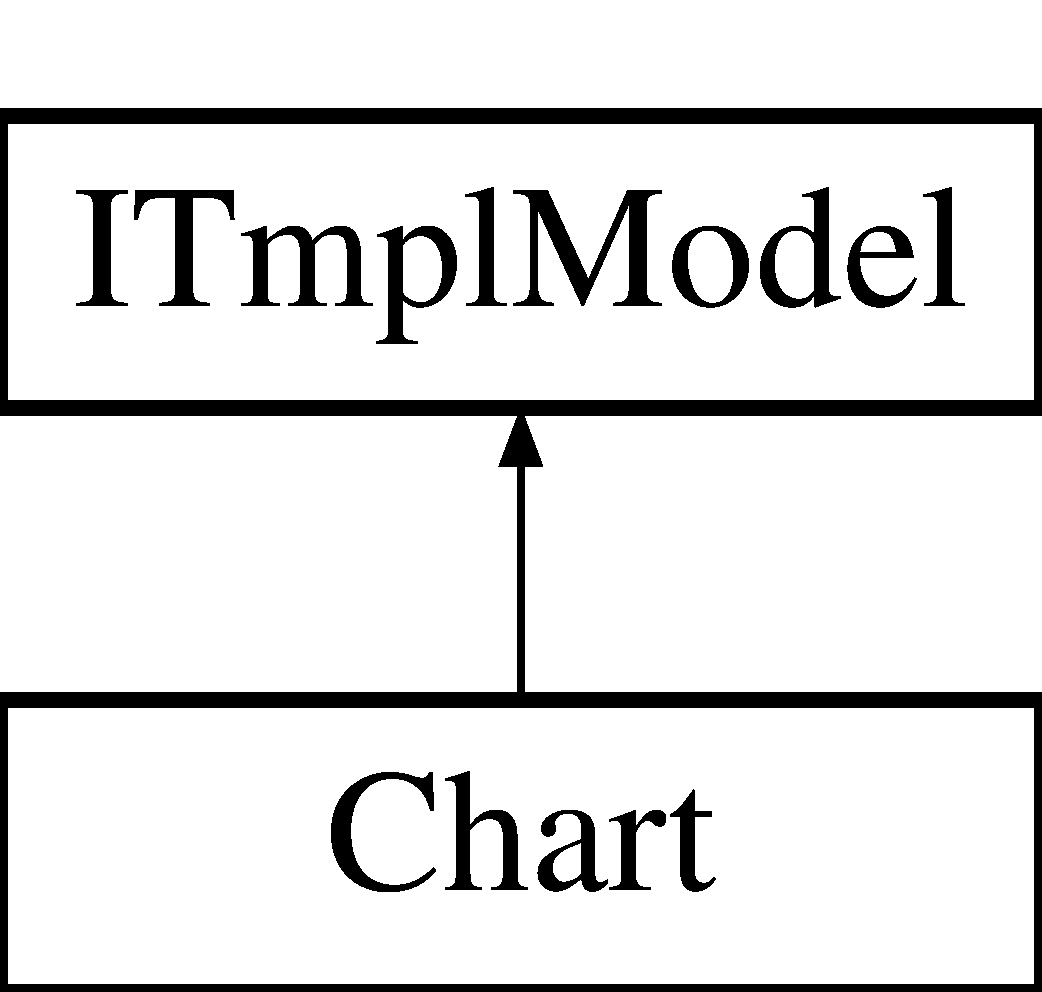
\includegraphics[height=2.000000cm]{classHighcharts_1_1Chart}
\end{center}
\end{figure}
\subsubsection*{Public Member Functions}
\begin{DoxyCompactItemize}
\item 
\mbox{\Hypertarget{classHighcharts_1_1Chart_a625845e2b8c6f042ff83d9db852e3f92}\label{classHighcharts_1_1Chart_a625845e2b8c6f042ff83d9db852e3f92}} 
{\bfseries Chart} (\hyperlink{classHighcharts_1_1Highchart}{Highchart} chart\+Type)
\item 
\mbox{\Hypertarget{classHighcharts_1_1Chart_a4fd34144f1927049fcfa878b7fed7415}\label{classHighcharts_1_1Chart_a4fd34144f1927049fcfa878b7fed7415}} 
void {\bfseries Set\+Div\+Id} (string divid)
\item 
\mbox{\Hypertarget{classHighcharts_1_1Chart_aafd35e8a8dfcb88c2c6bfb19aa8591a0}\label{classHighcharts_1_1Chart_aafd35e8a8dfcb88c2c6bfb19aa8591a0}} 
void {\bfseries Set\+Chart\+Type} (string type)
\item 
\mbox{\Hypertarget{classHighcharts_1_1Chart_a85d10a08b93b41e9696d777ec987f182}\label{classHighcharts_1_1Chart_a85d10a08b93b41e9696d777ec987f182}} 
void {\bfseries Set\+Title} (string title)
\item 
\mbox{\Hypertarget{classHighcharts_1_1Chart_aba272ac5f497b412f19590ed216f21f1}\label{classHighcharts_1_1Chart_aba272ac5f497b412f19590ed216f21f1}} 
void {\bfseries Set\+Subtitle} (string subtitle)
\item 
\mbox{\Hypertarget{classHighcharts_1_1Chart_a89a203b5d6bd81aec960ae3fb1fd4e17}\label{classHighcharts_1_1Chart_a89a203b5d6bd81aec960ae3fb1fd4e17}} 
void {\bfseries Set\+Xlabel} (string xlabel)
\item 
\mbox{\Hypertarget{classHighcharts_1_1Chart_ac009641d79c870f1b131faa30a740979}\label{classHighcharts_1_1Chart_ac009641d79c870f1b131faa30a740979}} 
void {\bfseries Set\+Ylabel} (string ylabel)
\item 
\mbox{\Hypertarget{classHighcharts_1_1Chart_a596a28a795aa22d8e8bc42a83c549529}\label{classHighcharts_1_1Chart_a596a28a795aa22d8e8bc42a83c549529}} 
void {\bfseries Set\+Xtooltip} (string xtooltip)
\item 
\mbox{\Hypertarget{classHighcharts_1_1Chart_a13b3b073d6debd31afdc6c4fe29a4a47}\label{classHighcharts_1_1Chart_a13b3b073d6debd31afdc6c4fe29a4a47}} 
void {\bfseries Set\+Ytooltip} (string ytooltip)
\item 
\mbox{\Hypertarget{classHighcharts_1_1Chart_a8de4430c7a4d26ca3ef2506c1ec4e9e9}\label{classHighcharts_1_1Chart_a8de4430c7a4d26ca3ef2506c1ec4e9e9}} 
string {\bfseries Create\+Template} ()
\item 
\mbox{\Hypertarget{classHighcharts_1_1Chart_ab740cbd7e41f8e63cb60d9b54357c654}\label{classHighcharts_1_1Chart_ab740cbd7e41f8e63cb60d9b54357c654}} 
void {\bfseries Add\+Data\+Series} (\hyperlink{classHighcharts_1_1DataSeries}{Data\+Series} data)
\item 
\mbox{\Hypertarget{classHighcharts_1_1Chart_a3d07ca3f01584223ab2ce140b8f14e5e}\label{classHighcharts_1_1Chart_a3d07ca3f01584223ab2ce140b8f14e5e}} 
List$<$ Tuple$<$ string, string $>$ $>$ {\bfseries Get\+Replacers} ()
\end{DoxyCompactItemize}
\subsubsection*{Properties}
\begin{DoxyCompactItemize}
\item 
\mbox{\Hypertarget{classHighcharts_1_1Chart_a5b6ed5b7cf2b4c06fcab23ae89e90697}\label{classHighcharts_1_1Chart_a5b6ed5b7cf2b4c06fcab23ae89e90697}} 
string {\bfseries Template} = \char`\"{}scatterplot\char`\"{}\hspace{0.3cm}{\ttfamily  \mbox{[}get\mbox{]}}
\end{DoxyCompactItemize}
\subsubsection*{Private Attributes}
\begin{DoxyCompactItemize}
\item 
\mbox{\Hypertarget{classHighcharts_1_1Chart_a2f6ad2d7ce597e1ca217d737983ff522}\label{classHighcharts_1_1Chart_a2f6ad2d7ce597e1ca217d737983ff522}} 
readonly Dictionary$<$ \hyperlink{classHighcharts_1_1Replacer}{Replacer}, string $>$ {\bfseries \+\_\+replacers} = new Dictionary$<$\hyperlink{classHighcharts_1_1Replacer}{Replacer}, string$>$()
\end{DoxyCompactItemize}

\hypertarget{classDataTools_1_1clustering_1_1ClusterPoint}{}\subsection{Data\+Tools.\+clustering.\+Cluster\+Point Class Reference}
\label{classDataTools_1_1clustering_1_1ClusterPoint}\index{Data\+Tools.\+clustering.\+Cluster\+Point@{Data\+Tools.\+clustering.\+Cluster\+Point}}


Vector that is assigned to a cluster.  


\subsubsection*{Public Member Functions}
\begin{DoxyCompactItemize}
\item 
\mbox{\Hypertarget{classDataTools_1_1clustering_1_1ClusterPoint_a91d0a96b0abb918424888f1a90e4c689}\label{classDataTools_1_1clustering_1_1ClusterPoint_a91d0a96b0abb918424888f1a90e4c689}} 
{\bfseries Cluster\+Point} (\hyperlink{classDataTools_1_1GenericVector}{Generic\+Vector} vector, int cluster=-\/1)
\end{DoxyCompactItemize}
\subsubsection*{Properties}
\begin{DoxyCompactItemize}
\item 
\mbox{\Hypertarget{classDataTools_1_1clustering_1_1ClusterPoint_affa614e6cc6858af01de3e04a7e9453d}\label{classDataTools_1_1clustering_1_1ClusterPoint_affa614e6cc6858af01de3e04a7e9453d}} 
bool {\bfseries Visited}\hspace{0.3cm}{\ttfamily  \mbox{[}get, set\mbox{]}}
\item 
\mbox{\Hypertarget{classDataTools_1_1clustering_1_1ClusterPoint_a6d6f1bc4e9f1aaacfdcb8f035c0b63a7}\label{classDataTools_1_1clustering_1_1ClusterPoint_a6d6f1bc4e9f1aaacfdcb8f035c0b63a7}} 
bool {\bfseries Noise}\hspace{0.3cm}{\ttfamily  \mbox{[}get, set\mbox{]}}
\item 
\mbox{\Hypertarget{classDataTools_1_1clustering_1_1ClusterPoint_a6f46873bc5cd699e62445c1e51b67d3c}\label{classDataTools_1_1clustering_1_1ClusterPoint_a6f46873bc5cd699e62445c1e51b67d3c}} 
\hyperlink{classDataTools_1_1GenericVector}{Generic\+Vector} {\bfseries Vector}\hspace{0.3cm}{\ttfamily  \mbox{[}get\mbox{]}}
\item 
\mbox{\Hypertarget{classDataTools_1_1clustering_1_1ClusterPoint_ae32ce03573ebee573a3cfd8d19648290}\label{classDataTools_1_1clustering_1_1ClusterPoint_ae32ce03573ebee573a3cfd8d19648290}} 
int {\bfseries Cluster}\hspace{0.3cm}{\ttfamily  \mbox{[}get, set\mbox{]}}
\end{DoxyCompactItemize}


\subsubsection{Detailed Description}
Vector that is assigned to a cluster. 

A \hyperlink{classDataTools_1_1clustering_1_1ClusterPoint}{Cluster\+Point} is a adapter that holds a \hyperlink{classDataTools_1_1GenericVector}{Generic\+Vector}, but adds some clusterting related properties to it. 

The documentation for this class was generated from the following file\+:\begin{DoxyCompactItemize}
\item 
Cluster\+Point.\+cs\end{DoxyCompactItemize}

\hypertarget{classDataTools_1_1correlation_1_1Correlation}{}\subsection{Correlation Class Reference}
\label{classDataTools_1_1correlation_1_1Correlation}\index{Correlation@{Correlation}}
Inheritance diagram for Correlation\+:\begin{figure}[H]
\begin{center}
\leavevmode
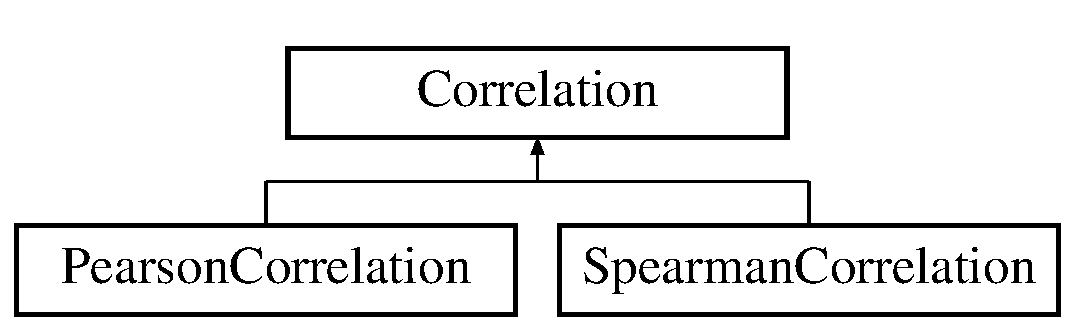
\includegraphics[height=2.000000cm]{classDataTools_1_1correlation_1_1Correlation}
\end{center}
\end{figure}
\subsubsection*{Public Member Functions}
\begin{DoxyCompactItemize}
\item 
\mbox{\Hypertarget{classDataTools_1_1correlation_1_1Correlation_aceb0beb9f4f7d80e96e8d94b20cdc823}\label{classDataTools_1_1correlation_1_1Correlation_aceb0beb9f4f7d80e96e8d94b20cdc823}} 
abstract double {\bfseries Get\+Correlation\+Coefficient} ()
\end{DoxyCompactItemize}
\subsubsection*{Protected Member Functions}
\begin{DoxyCompactItemize}
\item 
\mbox{\Hypertarget{classDataTools_1_1correlation_1_1Correlation_a9cfdaf3f9f7c45c8d50d127e144f22bb}\label{classDataTools_1_1correlation_1_1Correlation_a9cfdaf3f9f7c45c8d50d127e144f22bb}} 
{\bfseries Correlation} (I\+Enumerable$<$ \hyperlink{classDataTools_1_1Vector2}{Vector2} $>$ data)
\end{DoxyCompactItemize}
\subsubsection*{Protected Attributes}
\begin{DoxyCompactItemize}
\item 
\mbox{\Hypertarget{classDataTools_1_1correlation_1_1Correlation_a433eb6b10599d4c45f8df9022b2133c2}\label{classDataTools_1_1correlation_1_1Correlation_a433eb6b10599d4c45f8df9022b2133c2}} 
readonly I\+Enumerable$<$ \hyperlink{classDataTools_1_1Vector2}{Vector2} $>$ {\bfseries Data}
\end{DoxyCompactItemize}

\hypertarget{classHighcharts_1_1DataSeries}{}\subsection{Data\+Series Class Reference}
\label{classHighcharts_1_1DataSeries}\index{Data\+Series@{Data\+Series}}
Inheritance diagram for Data\+Series\+:\begin{figure}[H]
\begin{center}
\leavevmode
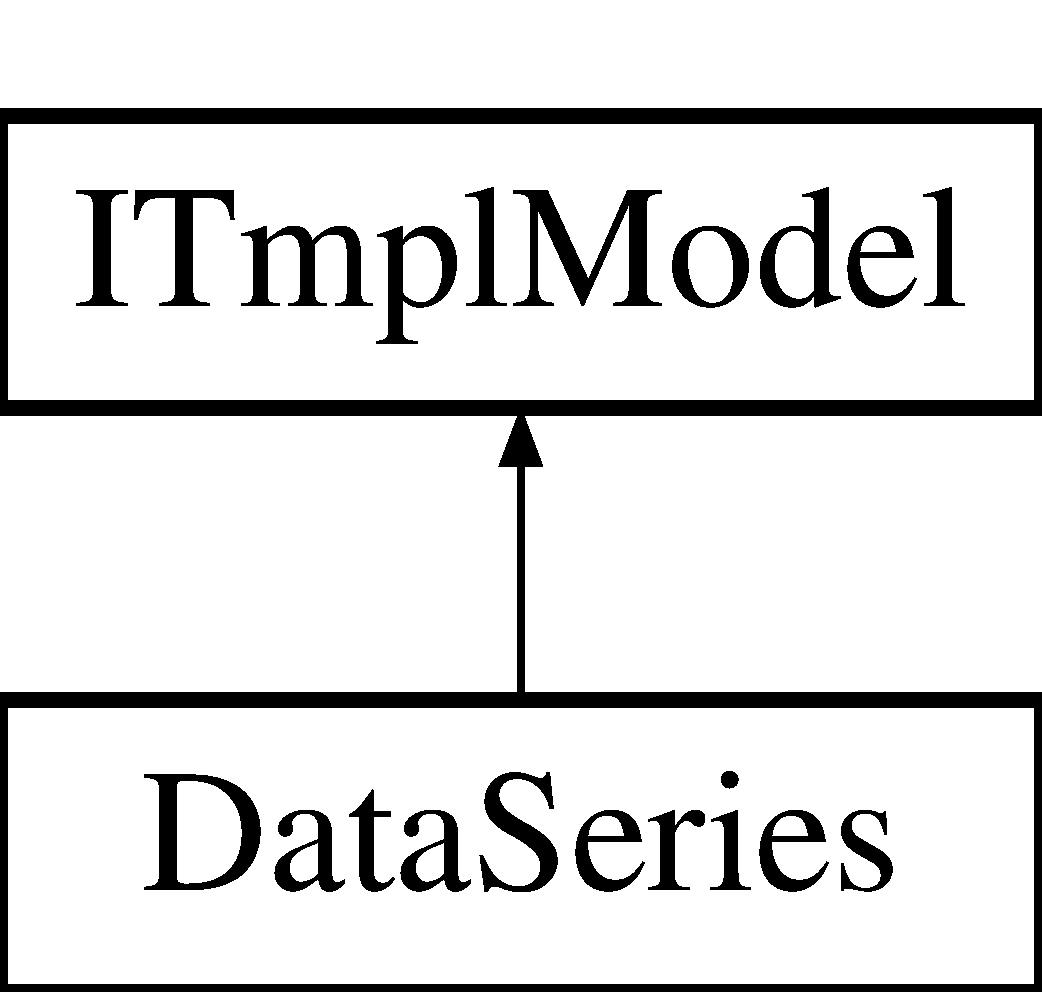
\includegraphics[height=2.000000cm]{classHighcharts_1_1DataSeries}
\end{center}
\end{figure}
\subsubsection*{Public Member Functions}
\begin{DoxyCompactItemize}
\item 
\mbox{\Hypertarget{classHighcharts_1_1DataSeries_a4dee11da81971b736dcdb922c49ee673}\label{classHighcharts_1_1DataSeries_a4dee11da81971b736dcdb922c49ee673}} 
{\bfseries Data\+Series} (\hyperlink{classHighcharts_1_1Highchart}{Highchart} type, \hyperlink{interfaceHighcharts_1_1IChartsList}{I\+Charts\+List} data, string name, bool marker=true, bool tracking=false)
\item 
\mbox{\Hypertarget{classHighcharts_1_1DataSeries_ac2e5653e93416c7de4fe29251c4470cd}\label{classHighcharts_1_1DataSeries_ac2e5653e93416c7de4fe29251c4470cd}} 
void {\bfseries Set\+Type} (string type)
\item 
\mbox{\Hypertarget{classHighcharts_1_1DataSeries_a82b23f1074f0c74e267aecd88a355a42}\label{classHighcharts_1_1DataSeries_a82b23f1074f0c74e267aecd88a355a42}} 
void {\bfseries Set\+Name} (string name)
\item 
\mbox{\Hypertarget{classHighcharts_1_1DataSeries_af44d67d2a2ce0f3ae4727b7cf501d245}\label{classHighcharts_1_1DataSeries_af44d67d2a2ce0f3ae4727b7cf501d245}} 
void {\bfseries Set\+Marker} (bool marker)
\item 
\mbox{\Hypertarget{classHighcharts_1_1DataSeries_a9bcedcb140286dd1987ccb2e18f27a6b}\label{classHighcharts_1_1DataSeries_a9bcedcb140286dd1987ccb2e18f27a6b}} 
void {\bfseries Set\+Mouse\+Tracking} (bool tracking)
\item 
\mbox{\Hypertarget{classHighcharts_1_1DataSeries_acd7d0fc170c47a8f8035ddd9eefca1df}\label{classHighcharts_1_1DataSeries_acd7d0fc170c47a8f8035ddd9eefca1df}} 
void {\bfseries Set\+Data} (\hyperlink{interfaceHighcharts_1_1IChartsList}{I\+Charts\+List} data)
\item 
\mbox{\Hypertarget{classHighcharts_1_1DataSeries_aeef147d554ea7643c83394f29297359e}\label{classHighcharts_1_1DataSeries_aeef147d554ea7643c83394f29297359e}} 
string {\bfseries To\+Tmpl\+String} ()
\item 
\mbox{\Hypertarget{classHighcharts_1_1DataSeries_a8de4430c7a4d26ca3ef2506c1ec4e9e9}\label{classHighcharts_1_1DataSeries_a8de4430c7a4d26ca3ef2506c1ec4e9e9}} 
string {\bfseries Create\+Template} ()
\item 
\mbox{\Hypertarget{classHighcharts_1_1DataSeries_a3d07ca3f01584223ab2ce140b8f14e5e}\label{classHighcharts_1_1DataSeries_a3d07ca3f01584223ab2ce140b8f14e5e}} 
List$<$ Tuple$<$ string, string $>$ $>$ {\bfseries Get\+Replacers} ()
\end{DoxyCompactItemize}
\subsubsection*{Properties}
\begin{DoxyCompactItemize}
\item 
\mbox{\Hypertarget{classHighcharts_1_1DataSeries_a5b6ed5b7cf2b4c06fcab23ae89e90697}\label{classHighcharts_1_1DataSeries_a5b6ed5b7cf2b4c06fcab23ae89e90697}} 
string {\bfseries Template} = \char`\"{}dataseries\char`\"{}\hspace{0.3cm}{\ttfamily  \mbox{[}get\mbox{]}}
\end{DoxyCompactItemize}
\subsubsection*{Private Attributes}
\begin{DoxyCompactItemize}
\item 
\mbox{\Hypertarget{classHighcharts_1_1DataSeries_a2f6ad2d7ce597e1ca217d737983ff522}\label{classHighcharts_1_1DataSeries_a2f6ad2d7ce597e1ca217d737983ff522}} 
readonly Dictionary$<$ \hyperlink{classHighcharts_1_1Replacer}{Replacer}, string $>$ {\bfseries \+\_\+replacers} = new Dictionary$<$\hyperlink{classHighcharts_1_1Replacer}{Replacer}, string$>$()
\end{DoxyCompactItemize}

\hypertarget{classDataTools_1_1clustering_1_1Dbscan}{}\subsection{Dbscan Class Reference}
\label{classDataTools_1_1clustering_1_1Dbscan}\index{Dbscan@{Dbscan}}


Class featuring the DB Scan algorithm.  


\subsubsection*{Public Member Functions}
\begin{DoxyCompactItemize}
\item 
\hyperlink{classDataTools_1_1clustering_1_1Dbscan_ac54fa4e699ed60d33e90b0deab9f4006_ac54fa4e699ed60d33e90b0deab9f4006}{Dbscan} (float eps, int min\+Points, I\+Enumerable$<$ \hyperlink{classDataTools_1_1GenericVector}{Generic\+Vector} $>$ data)
\end{DoxyCompactItemize}
\subsubsection*{Properties}
\begin{DoxyCompactItemize}
\item 
\mbox{\Hypertarget{classDataTools_1_1clustering_1_1Dbscan_a06317119faad60c7efd9feabeb13c795}\label{classDataTools_1_1clustering_1_1Dbscan_a06317119faad60c7efd9feabeb13c795}} 
Dictionary$<$ int, I\+Enumerable$<$ \hyperlink{classDataTools_1_1GenericVector}{Generic\+Vector} $>$ $>$ {\bfseries Data\+Clusters}\hspace{0.3cm}{\ttfamily  \mbox{[}get\mbox{]}}
\end{DoxyCompactItemize}


\subsubsection{Detailed Description}
Class featuring the DB Scan algorithm. 

The DB Scan algorithm is capable of clustering vectors of {\ttfamily n} dimensions. As input, it needs a radius within neighbours should be together, the minimum amount of point in a cluster and ofcourse the dataset, in this case, a {\ttfamily I\+Enumerable$<$\+Generic\+Vector$>$}. As output it produces a Dictionary Data\+Clusters with the key as cluster and the value the vectors belonging to the cluster. 

\subsubsection{Constructor \& Destructor Documentation}
\mbox{\Hypertarget{classDataTools_1_1clustering_1_1Dbscan_ac54fa4e699ed60d33e90b0deab9f4006_ac54fa4e699ed60d33e90b0deab9f4006}\label{classDataTools_1_1clustering_1_1Dbscan_ac54fa4e699ed60d33e90b0deab9f4006_ac54fa4e699ed60d33e90b0deab9f4006}} 
\index{Data\+Tools\+::clustering\+::\+Dbscan@{Data\+Tools\+::clustering\+::\+Dbscan}!Dbscan@{Dbscan}}
\index{Dbscan@{Dbscan}!Data\+Tools\+::clustering\+::\+Dbscan@{Data\+Tools\+::clustering\+::\+Dbscan}}
\paragraph{\texorpdfstring{Dbscan()}{Dbscan()}}
{\footnotesize\ttfamily \hyperlink{classDataTools_1_1clustering_1_1Dbscan}{Dbscan} (\begin{DoxyParamCaption}\item[{float}]{eps,  }\item[{int}]{min\+Points,  }\item[{I\+Enumerable$<$ \hyperlink{classDataTools_1_1GenericVector}{Generic\+Vector} $>$}]{data }\end{DoxyParamCaption})}

Constructor for DB Scan 
\begin{DoxyParams}{Parameters}
{\em eps} & Radius within neighbours should be \\
\hline
{\em min\+Points} & Min amount of points in a cluster \\
\hline
{\em data} & Dataset to cluster \\
\hline
\end{DoxyParams}

\hypertarget{classTree_1_1Empty}{}\subsection{Empty$<$ T $>$ Class Template Reference}
\label{classTree_1_1Empty}\index{Empty$<$ T $>$@{Empty$<$ T $>$}}
Inheritance diagram for Empty$<$ T $>$\+:\begin{figure}[H]
\begin{center}
\leavevmode
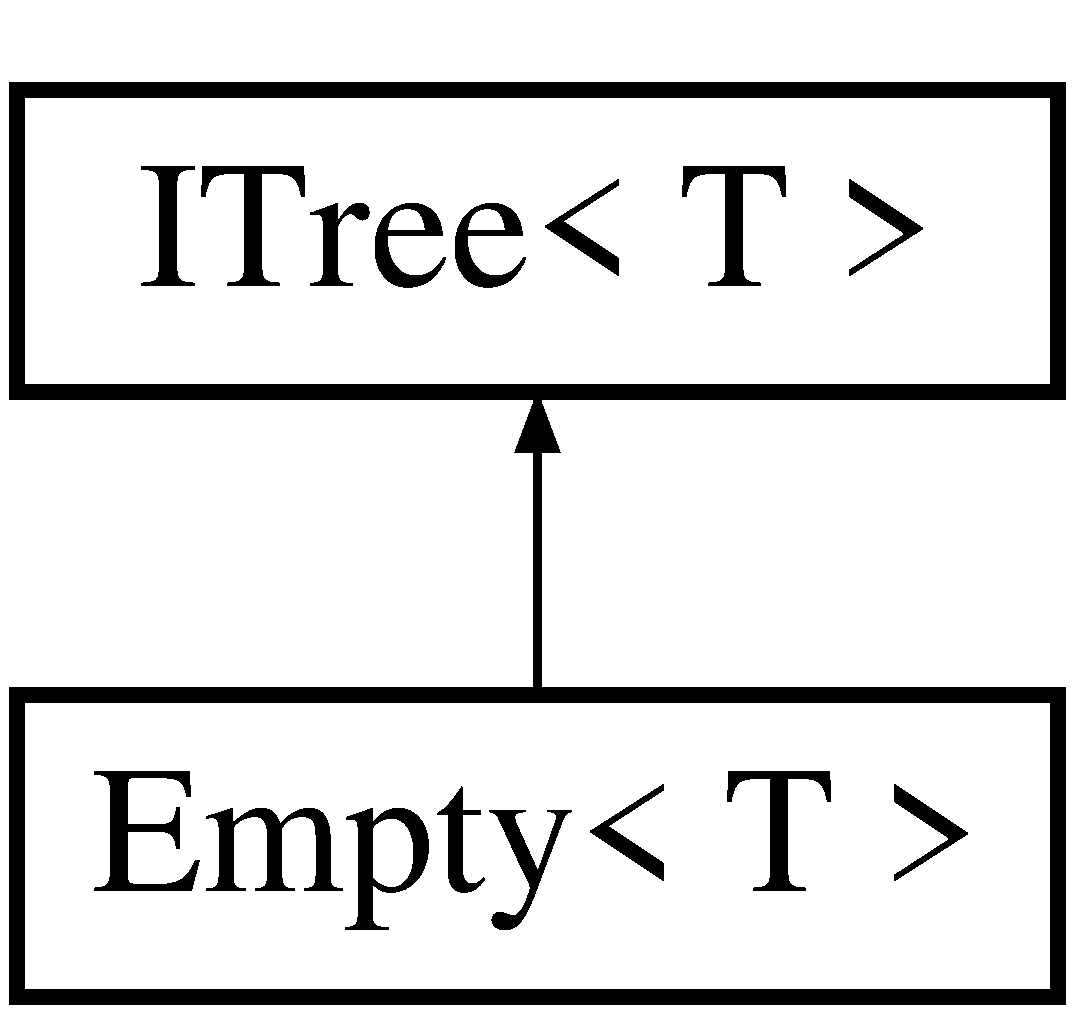
\includegraphics[height=2.000000cm]{classTree_1_1Empty}
\end{center}
\end{figure}
\subsubsection*{Public Attributes}
\begin{DoxyCompactItemize}
\item 
\mbox{\Hypertarget{classTree_1_1Empty_aaaa6c7dd3bd14dc2ce7f0780de528bb1}\label{classTree_1_1Empty_aaaa6c7dd3bd14dc2ce7f0780de528bb1}} 
bool {\bfseries Is\+Empty} =$>$ false
\end{DoxyCompactItemize}
\subsubsection*{Properties}
\begin{DoxyCompactItemize}
\item 
\mbox{\Hypertarget{classTree_1_1Empty_a9fa96587382d530a02e7e15b047e82ee}\label{classTree_1_1Empty_a9fa96587382d530a02e7e15b047e82ee}} 
int {\bfseries Dimension}\hspace{0.3cm}{\ttfamily  \mbox{[}get\mbox{]}}
\item 
\mbox{\Hypertarget{classTree_1_1Empty_ab08dc0c825bf3d24d4a6f9d238faaefb}\label{classTree_1_1Empty_ab08dc0c825bf3d24d4a6f9d238faaefb}} 
\hyperlink{interfaceTree_1_1ITree}{I\+Tree}$<$ T $>$ {\bfseries Left}\hspace{0.3cm}{\ttfamily  \mbox{[}get\mbox{]}}
\item 
\mbox{\Hypertarget{classTree_1_1Empty_ad438dde947eb8d4fa0b73ebb3d7973e9}\label{classTree_1_1Empty_ad438dde947eb8d4fa0b73ebb3d7973e9}} 
\hyperlink{interfaceTree_1_1ITree}{I\+Tree}$<$ T $>$ {\bfseries Right}\hspace{0.3cm}{\ttfamily  \mbox{[}get\mbox{]}}
\item 
\mbox{\Hypertarget{classTree_1_1Empty_adbfa996292c448f754363aa83d4be8e6}\label{classTree_1_1Empty_adbfa996292c448f754363aa83d4be8e6}} 
T {\bfseries Value}\hspace{0.3cm}{\ttfamily  \mbox{[}get\mbox{]}}
\end{DoxyCompactItemize}

\hypertarget{classDataTools_1_1GenericVector}{}\subsection{Generic\+Vector Class Reference}
\label{classDataTools_1_1GenericVector}\index{Generic\+Vector@{Generic\+Vector}}


N dimensional vector.  


\subsubsection*{Public Member Functions}
\begin{DoxyCompactItemize}
\item 
\mbox{\Hypertarget{classDataTools_1_1GenericVector_aaa9bcf132f1691298b9bb672f22787d2}\label{classDataTools_1_1GenericVector_aaa9bcf132f1691298b9bb672f22787d2}} 
{\bfseries Generic\+Vector} (int size)
\item 
\mbox{\Hypertarget{classDataTools_1_1GenericVector_a542ba2abc2b5ad8a398ad97bf2a682b0}\label{classDataTools_1_1GenericVector_a542ba2abc2b5ad8a398ad97bf2a682b0}} 
{\bfseries Generic\+Vector} (params double\mbox{[}$\,$\mbox{]} args)
\item 
\mbox{\Hypertarget{classDataTools_1_1GenericVector_adf109e0e2008229e56ef6f898425311d}\label{classDataTools_1_1GenericVector_adf109e0e2008229e56ef6f898425311d}} 
double \mbox{[}$\,$\mbox{]} {\bfseries To\+Array} ()
\item 
\mbox{\Hypertarget{classDataTools_1_1GenericVector_aa73e7c4dd1df5fd5fbf81c7764ee1533}\label{classDataTools_1_1GenericVector_aa73e7c4dd1df5fd5fbf81c7764ee1533}} 
override string {\bfseries To\+String} ()
\item 
\mbox{\Hypertarget{classDataTools_1_1GenericVector_a31e1a43cd76a962c919d06400fdcc10b}\label{classDataTools_1_1GenericVector_a31e1a43cd76a962c919d06400fdcc10b}} 
\hyperlink{classDataTools_1_1Vector2}{Vector2} {\bfseries To\+Vector2} (int index\+One=0, int index\+Two=1)
\end{DoxyCompactItemize}
\subsubsection*{Static Public Member Functions}
\begin{DoxyCompactItemize}
\item 
\mbox{\Hypertarget{classDataTools_1_1GenericVector_af0e039764e63ac4045ae9946c22876b7}\label{classDataTools_1_1GenericVector_af0e039764e63ac4045ae9946c22876b7}} 
static \hyperlink{classDataTools_1_1GenericVector}{Generic\+Vector} {\bfseries Sum} (\hyperlink{classDataTools_1_1GenericVector}{Generic\+Vector} a, \hyperlink{classDataTools_1_1GenericVector}{Generic\+Vector} b)
\item 
\mbox{\Hypertarget{classDataTools_1_1GenericVector_a4d4381024a0923328a212e567f5f3a65}\label{classDataTools_1_1GenericVector_a4d4381024a0923328a212e567f5f3a65}} 
static \hyperlink{classDataTools_1_1GenericVector}{Generic\+Vector} {\bfseries Devide} (\hyperlink{classDataTools_1_1GenericVector}{Generic\+Vector} a, int devider)
\item 
\mbox{\Hypertarget{classDataTools_1_1GenericVector_ab2af09a4dcf0d49252e0a388de75b1a6}\label{classDataTools_1_1GenericVector_ab2af09a4dcf0d49252e0a388de75b1a6}} 
static double {\bfseries Distance} (\hyperlink{classDataTools_1_1GenericVector}{Generic\+Vector} a, \hyperlink{classDataTools_1_1GenericVector}{Generic\+Vector} b)
\end{DoxyCompactItemize}
\subsubsection*{Public Attributes}
\begin{DoxyCompactItemize}
\item 
\mbox{\Hypertarget{classDataTools_1_1GenericVector_af06eb7b9b70be91dadd4f12ebcaed796}\label{classDataTools_1_1GenericVector_af06eb7b9b70be91dadd4f12ebcaed796}} 
int {\bfseries Size} =$>$ \+\_\+points.\+Length
\item 
\mbox{\Hypertarget{classDataTools_1_1GenericVector_ab9334ca30e9ffb3ef0406a11c712f05c}\label{classDataTools_1_1GenericVector_ab9334ca30e9ffb3ef0406a11c712f05c}} 
double {\bfseries Biggest\+Point} =$>$ \+\_\+points.\+Max()
\item 
\mbox{\Hypertarget{classDataTools_1_1GenericVector_a18bad8396584a2fd063e49ba30a84d55}\label{classDataTools_1_1GenericVector_a18bad8396584a2fd063e49ba30a84d55}} 
double {\bfseries this\mbox{[}int x\mbox{]}} =$>$ \+\_\+points\mbox{[}x\mbox{]}
\end{DoxyCompactItemize}
\subsubsection*{Private Attributes}
\begin{DoxyCompactItemize}
\item 
\mbox{\Hypertarget{classDataTools_1_1GenericVector_ac05213eecd8c2fa58764505999b2fe36}\label{classDataTools_1_1GenericVector_ac05213eecd8c2fa58764505999b2fe36}} 
readonly double \mbox{[}$\,$\mbox{]} {\bfseries \+\_\+points}
\end{DoxyCompactItemize}


\subsubsection{Detailed Description}
N dimensional vector. 

This class is a vector with N dimensions. The amount of dimensions is created upon initialization and can not be changed afterwards. It implements some basic vector algebra like summation, multiplication and deviding. 
\hypertarget{classHighcharts_1_1Highchart}{}\subsection{Highchart Class Reference}
\label{classHighcharts_1_1Highchart}\index{Highchart@{Highchart}}
\subsubsection*{Static Public Attributes}
\begin{DoxyCompactItemize}
\item 
\mbox{\Hypertarget{classHighcharts_1_1Highchart_a152d250f31b12e9713ed04fd672c95a8}\label{classHighcharts_1_1Highchart_a152d250f31b12e9713ed04fd672c95a8}} 
static readonly \hyperlink{classHighcharts_1_1Highchart}{Highchart} {\bfseries Scatterplot} = new \hyperlink{classHighcharts_1_1Highchart}{Highchart}(\char`\"{}scatter\char`\"{})
\item 
\mbox{\Hypertarget{classHighcharts_1_1Highchart_a9ec66595aaa01595731452d18ed8a402}\label{classHighcharts_1_1Highchart_a9ec66595aaa01595731452d18ed8a402}} 
static readonly \hyperlink{classHighcharts_1_1Highchart}{Highchart} {\bfseries Regression} = new \hyperlink{classHighcharts_1_1Highchart}{Highchart}(\char`\"{}line\char`\"{})
\end{DoxyCompactItemize}
\subsubsection*{Properties}
\begin{DoxyCompactItemize}
\item 
\mbox{\Hypertarget{classHighcharts_1_1Highchart_af7b88db799d8f791f785e437bc6099d2}\label{classHighcharts_1_1Highchart_af7b88db799d8f791f785e437bc6099d2}} 
string {\bfseries Value}\hspace{0.3cm}{\ttfamily  \mbox{[}get\mbox{]}}
\end{DoxyCompactItemize}
\subsubsection*{Private Member Functions}
\begin{DoxyCompactItemize}
\item 
\mbox{\Hypertarget{classHighcharts_1_1Highchart_a15fc3de64317e04fa3642ed4bf0b2797}\label{classHighcharts_1_1Highchart_a15fc3de64317e04fa3642ed4bf0b2797}} 
{\bfseries Highchart} (string value)
\end{DoxyCompactItemize}

\hypertarget{interfaceHighcharts_1_1IChartsList}{}\subsection{I\+Charts\+List Interface Reference}
\label{interfaceHighcharts_1_1IChartsList}\index{I\+Charts\+List@{I\+Charts\+List}}
\subsubsection*{Public Member Functions}
\begin{DoxyCompactItemize}
\item 
\mbox{\Hypertarget{interfaceHighcharts_1_1IChartsList_ae5263ba3c7ada40ab2538080496e8bf0}\label{interfaceHighcharts_1_1IChartsList_ae5263ba3c7ada40ab2538080496e8bf0}} 
string {\bfseries To\+Charts\+List} ()
\end{DoxyCompactItemize}

\hypertarget{interfaceHighcharts_1_1ITmplModel}{}\subsection{I\+Tmpl\+Model Interface Reference}
\label{interfaceHighcharts_1_1ITmplModel}\index{I\+Tmpl\+Model@{I\+Tmpl\+Model}}
Inheritance diagram for I\+Tmpl\+Model\+:\begin{figure}[H]
\begin{center}
\leavevmode
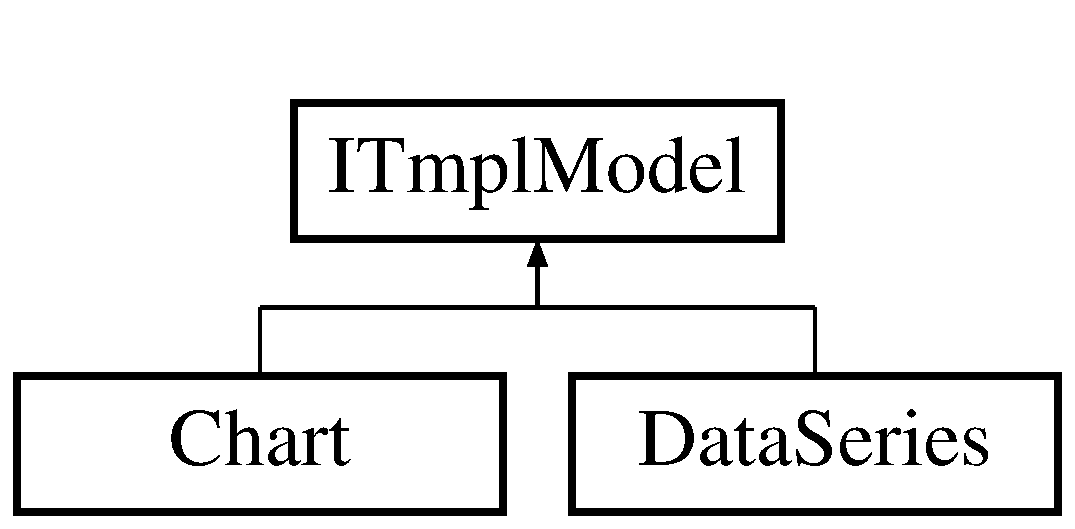
\includegraphics[height=2.000000cm]{interfaceHighcharts_1_1ITmplModel}
\end{center}
\end{figure}
\subsubsection*{Public Member Functions}
\begin{DoxyCompactItemize}
\item 
\mbox{\Hypertarget{interfaceHighcharts_1_1ITmplModel_a8de4430c7a4d26ca3ef2506c1ec4e9e9}\label{interfaceHighcharts_1_1ITmplModel_a8de4430c7a4d26ca3ef2506c1ec4e9e9}} 
string {\bfseries Create\+Template} ()
\item 
\mbox{\Hypertarget{interfaceHighcharts_1_1ITmplModel_a3d07ca3f01584223ab2ce140b8f14e5e}\label{interfaceHighcharts_1_1ITmplModel_a3d07ca3f01584223ab2ce140b8f14e5e}} 
List$<$ Tuple$<$ string, string $>$ $>$ {\bfseries Get\+Replacers} ()
\end{DoxyCompactItemize}
\subsubsection*{Properties}
\begin{DoxyCompactItemize}
\item 
\mbox{\Hypertarget{interfaceHighcharts_1_1ITmplModel_a5b6ed5b7cf2b4c06fcab23ae89e90697}\label{interfaceHighcharts_1_1ITmplModel_a5b6ed5b7cf2b4c06fcab23ae89e90697}} 
string {\bfseries Template}\hspace{0.3cm}{\ttfamily  \mbox{[}get\mbox{]}}
\end{DoxyCompactItemize}

\hypertarget{interfaceTree_1_1ITree}{}\subsection{I\+Tree$<$ T $>$ Interface Template Reference}
\label{interfaceTree_1_1ITree}\index{I\+Tree$<$ T $>$@{I\+Tree$<$ T $>$}}
Inheritance diagram for I\+Tree$<$ T $>$\+:\begin{figure}[H]
\begin{center}
\leavevmode
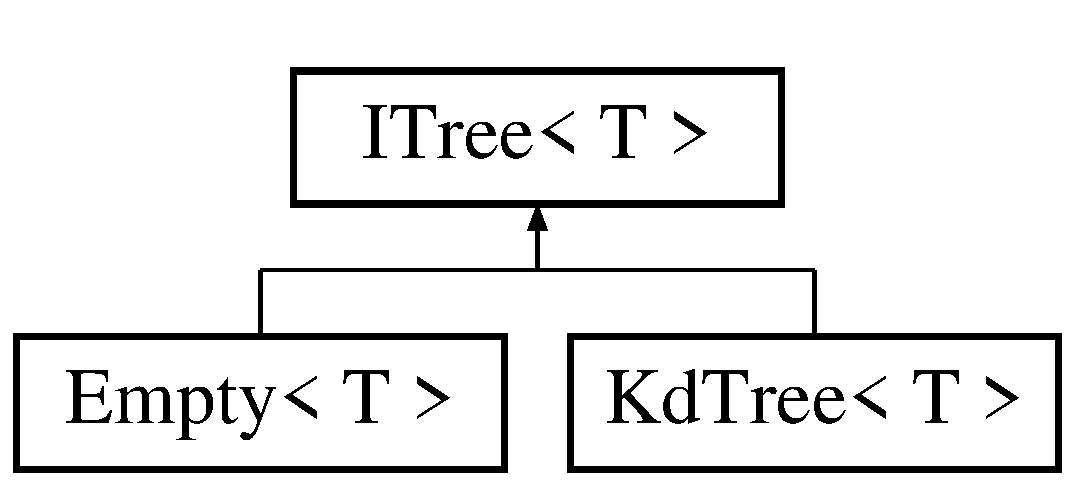
\includegraphics[height=2.000000cm]{interfaceTree_1_1ITree}
\end{center}
\end{figure}
\subsubsection*{Properties}
\begin{DoxyCompactItemize}
\item 
\mbox{\Hypertarget{interfaceTree_1_1ITree_a9fa96587382d530a02e7e15b047e82ee}\label{interfaceTree_1_1ITree_a9fa96587382d530a02e7e15b047e82ee}} 
int {\bfseries Dimension}\hspace{0.3cm}{\ttfamily  \mbox{[}get\mbox{]}}
\item 
\mbox{\Hypertarget{interfaceTree_1_1ITree_ab08dc0c825bf3d24d4a6f9d238faaefb}\label{interfaceTree_1_1ITree_ab08dc0c825bf3d24d4a6f9d238faaefb}} 
\hyperlink{interfaceTree_1_1ITree}{I\+Tree}$<$ T $>$ {\bfseries Left}\hspace{0.3cm}{\ttfamily  \mbox{[}get\mbox{]}}
\item 
\mbox{\Hypertarget{interfaceTree_1_1ITree_ad438dde947eb8d4fa0b73ebb3d7973e9}\label{interfaceTree_1_1ITree_ad438dde947eb8d4fa0b73ebb3d7973e9}} 
\hyperlink{interfaceTree_1_1ITree}{I\+Tree}$<$ T $>$ {\bfseries Right}\hspace{0.3cm}{\ttfamily  \mbox{[}get\mbox{]}}
\item 
\mbox{\Hypertarget{interfaceTree_1_1ITree_adbfa996292c448f754363aa83d4be8e6}\label{interfaceTree_1_1ITree_adbfa996292c448f754363aa83d4be8e6}} 
T {\bfseries Value}\hspace{0.3cm}{\ttfamily  \mbox{[}get\mbox{]}}
\item 
\mbox{\Hypertarget{interfaceTree_1_1ITree_aaaa6c7dd3bd14dc2ce7f0780de528bb1}\label{interfaceTree_1_1ITree_aaaa6c7dd3bd14dc2ce7f0780de528bb1}} 
bool {\bfseries Is\+Empty}\hspace{0.3cm}{\ttfamily  \mbox{[}get\mbox{]}}
\end{DoxyCompactItemize}

\hypertarget{classTree_1_1KdTree}{}\subsection{Kd\+Tree$<$ T $>$ Class Template Reference}
\label{classTree_1_1KdTree}\index{Kd\+Tree$<$ T $>$@{Kd\+Tree$<$ T $>$}}
Inheritance diagram for Kd\+Tree$<$ T $>$\+:\begin{figure}[H]
\begin{center}
\leavevmode
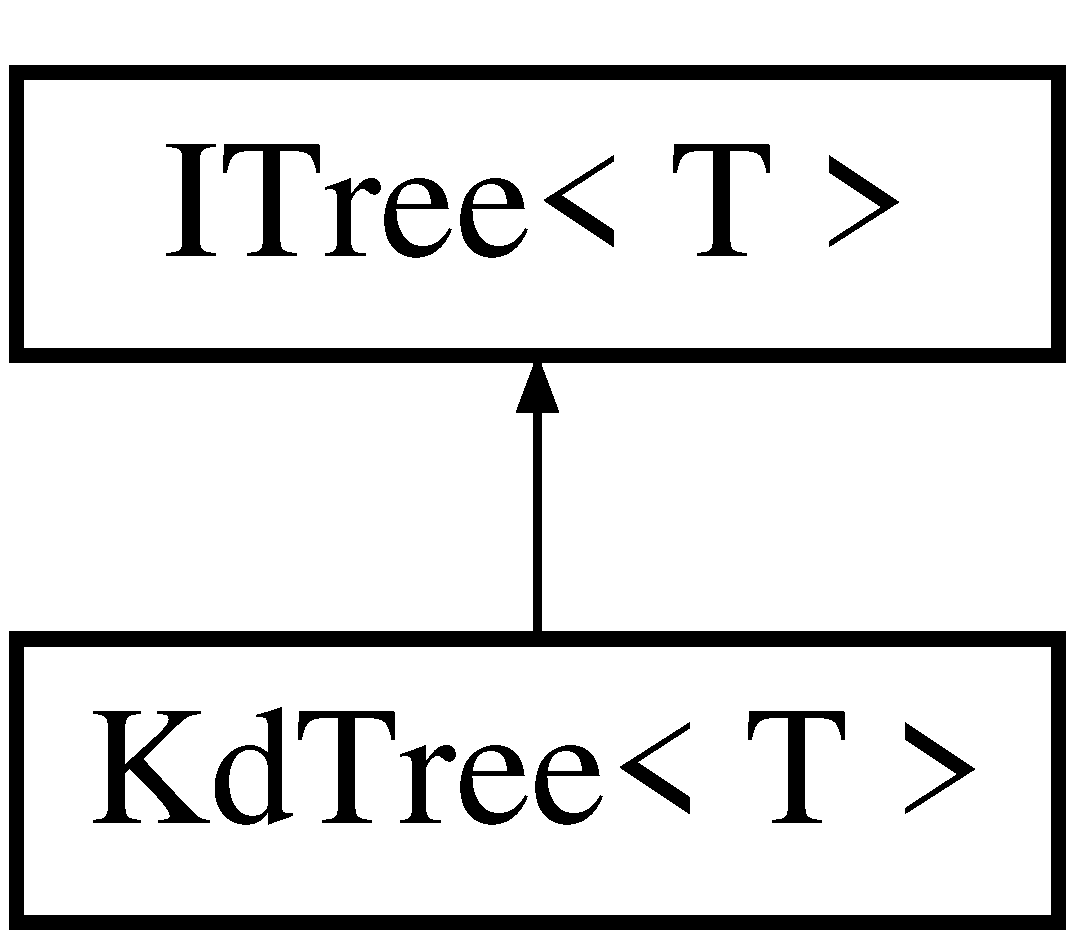
\includegraphics[height=2.000000cm]{classTree_1_1KdTree}
\end{center}
\end{figure}
\subsubsection*{Public Attributes}
\begin{DoxyCompactItemize}
\item 
\mbox{\Hypertarget{classTree_1_1KdTree_aaaa6c7dd3bd14dc2ce7f0780de528bb1}\label{classTree_1_1KdTree_aaaa6c7dd3bd14dc2ce7f0780de528bb1}} 
bool {\bfseries Is\+Empty} =$>$ true
\end{DoxyCompactItemize}
\subsubsection*{Protected Member Functions}
\begin{DoxyCompactItemize}
\item 
\mbox{\Hypertarget{classTree_1_1KdTree_a37d04aebfbb87df89283087fff07f7df}\label{classTree_1_1KdTree_a37d04aebfbb87df89283087fff07f7df}} 
{\bfseries Kd\+Tree} (\hyperlink{interfaceTree_1_1ITree}{I\+Tree}$<$ T $>$ left, T value, \hyperlink{interfaceTree_1_1ITree}{I\+Tree}$<$ T $>$ right, int dimension)
\end{DoxyCompactItemize}
\subsubsection*{Properties}
\begin{DoxyCompactItemize}
\item 
\mbox{\Hypertarget{classTree_1_1KdTree_a9fa96587382d530a02e7e15b047e82ee}\label{classTree_1_1KdTree_a9fa96587382d530a02e7e15b047e82ee}} 
int {\bfseries Dimension}\hspace{0.3cm}{\ttfamily  \mbox{[}get\mbox{]}}
\item 
\mbox{\Hypertarget{classTree_1_1KdTree_ab08dc0c825bf3d24d4a6f9d238faaefb}\label{classTree_1_1KdTree_ab08dc0c825bf3d24d4a6f9d238faaefb}} 
\hyperlink{interfaceTree_1_1ITree}{I\+Tree}$<$ T $>$ {\bfseries Left}\hspace{0.3cm}{\ttfamily  \mbox{[}get\mbox{]}}
\item 
\mbox{\Hypertarget{classTree_1_1KdTree_ad438dde947eb8d4fa0b73ebb3d7973e9}\label{classTree_1_1KdTree_ad438dde947eb8d4fa0b73ebb3d7973e9}} 
\hyperlink{interfaceTree_1_1ITree}{I\+Tree}$<$ T $>$ {\bfseries Right}\hspace{0.3cm}{\ttfamily  \mbox{[}get\mbox{]}}
\item 
\mbox{\Hypertarget{classTree_1_1KdTree_adbfa996292c448f754363aa83d4be8e6}\label{classTree_1_1KdTree_adbfa996292c448f754363aa83d4be8e6}} 
T {\bfseries Value}\hspace{0.3cm}{\ttfamily  \mbox{[}get\mbox{]}}
\end{DoxyCompactItemize}

\hypertarget{classDataTools_1_1clustering_1_1Kmeans}{}\subsection{Kmeans Class Reference}
\label{classDataTools_1_1clustering_1_1Kmeans}\index{Kmeans@{Kmeans}}


Class featuring de K\+Means algorithm.  


\subsubsection*{Public Member Functions}
\begin{DoxyCompactItemize}
\item 
\hyperlink{classDataTools_1_1clustering_1_1Kmeans_a0104b68b82ac185d65d0df9a02569ec8_a0104b68b82ac185d65d0df9a02569ec8}{Kmeans} (int k, int iterations, I\+Enumerable$<$ \hyperlink{classDataTools_1_1GenericVector}{Generic\+Vector} $>$ data\+Set)
\end{DoxyCompactItemize}
\subsubsection*{Properties}
\begin{DoxyCompactItemize}
\item 
\mbox{\Hypertarget{classDataTools_1_1clustering_1_1Kmeans_a06317119faad60c7efd9feabeb13c795}\label{classDataTools_1_1clustering_1_1Kmeans_a06317119faad60c7efd9feabeb13c795}} 
Dictionary$<$ int, I\+Enumerable$<$ \hyperlink{classDataTools_1_1GenericVector}{Generic\+Vector} $>$ $>$ {\bfseries Data\+Clusters}\hspace{0.3cm}{\ttfamily  \mbox{[}get\mbox{]}}
\end{DoxyCompactItemize}
\subsubsection*{Private Member Functions}
\begin{DoxyCompactItemize}
\item 
void \hyperlink{classDataTools_1_1clustering_1_1Kmeans_aa3eca255b6be227d7d901cc2a72017a5_aa3eca255b6be227d7d901cc2a72017a5}{Run} ()
\item 
void \hyperlink{classDataTools_1_1clustering_1_1Kmeans_a348b17d6f4e97ca727ba1c9dad533d2b_a348b17d6f4e97ca727ba1c9dad533d2b}{Recalculate\+Clusters} ()
\item 
void \hyperlink{classDataTools_1_1clustering_1_1Kmeans_a7fff9b4f946273bc93e33a468c23d1a8_a7fff9b4f946273bc93e33a468c23d1a8}{Recalculate\+Centroids} ()
\item 
int \hyperlink{classDataTools_1_1clustering_1_1Kmeans_a0b0bf52405efb95800cf147176b85c4e_a0b0bf52405efb95800cf147176b85c4e}{Get\+Nearest\+Cluster} (\hyperlink{classDataTools_1_1GenericVector}{Generic\+Vector} v)
\item 
Dictionary$<$ int, \hyperlink{classDataTools_1_1GenericVector}{Generic\+Vector} $>$ \hyperlink{classDataTools_1_1clustering_1_1Kmeans_a9000ebd9a16ff504a2a0ffb139871fba_a9000ebd9a16ff504a2a0ffb139871fba}{Generate\+Random\+Centroids} (int k\+Amount)
\item 
\hyperlink{classDataTools_1_1GenericVector}{Generic\+Vector} \hyperlink{classDataTools_1_1clustering_1_1Kmeans_adb45b460ab8312abb30b509c15fd91fb_adb45b460ab8312abb30b509c15fd91fb}{Get\+Random\+Vector} ()
\end{DoxyCompactItemize}
\subsubsection*{Static Private Member Functions}
\begin{DoxyCompactItemize}
\item 
static bool \hyperlink{classDataTools_1_1clustering_1_1Kmeans_a9347cabe7e34cd6847d27df3d275195d_a9347cabe7e34cd6847d27df3d275195d}{Is\+Changed\+Cluster} (I\+Enumerable$<$ int $>$ a, I\+Read\+Only\+List$<$ int $>$ b)
\end{DoxyCompactItemize}
\subsubsection*{Private Attributes}
\begin{DoxyCompactItemize}
\item 
\mbox{\Hypertarget{classDataTools_1_1clustering_1_1Kmeans_a0a5c3bc889cf50b80ab55ebed8f57312}\label{classDataTools_1_1clustering_1_1Kmeans_a0a5c3bc889cf50b80ab55ebed8f57312}} 
readonly Random {\bfseries \+\_\+random} = new Random()
\item 
\mbox{\Hypertarget{classDataTools_1_1clustering_1_1Kmeans_a554eac85df5a5531150341dc478c63fa}\label{classDataTools_1_1clustering_1_1Kmeans_a554eac85df5a5531150341dc478c63fa}} 
readonly int {\bfseries \+\_\+clusters}
\item 
\mbox{\Hypertarget{classDataTools_1_1clustering_1_1Kmeans_a430bead482bd81bdb5197d3685bcdd0f}\label{classDataTools_1_1clustering_1_1Kmeans_a430bead482bd81bdb5197d3685bcdd0f}} 
readonly int {\bfseries \+\_\+iterations}
\item 
\mbox{\Hypertarget{classDataTools_1_1clustering_1_1Kmeans_a91e409ed78afae05248478bc0fb5445b}\label{classDataTools_1_1clustering_1_1Kmeans_a91e409ed78afae05248478bc0fb5445b}} 
readonly List$<$ \hyperlink{classDataTools_1_1clustering_1_1ClusterPoint}{Cluster\+Point} $>$ {\bfseries \+\_\+data\+Set}
\item 
\mbox{\Hypertarget{classDataTools_1_1clustering_1_1Kmeans_a736320ca5ab8246e8923f4c627ca058d}\label{classDataTools_1_1clustering_1_1Kmeans_a736320ca5ab8246e8923f4c627ca058d}} 
Dictionary$<$ int, \hyperlink{classDataTools_1_1GenericVector}{Generic\+Vector} $>$ {\bfseries \+\_\+centroids}
\end{DoxyCompactItemize}


\subsubsection{Detailed Description}
Class featuring de K\+Means algorithm. 

K\+Means is a clustering algorithm. As input it needs {\ttfamily k} (the amount of clusters), the max amount of iterations and the dataset to cluster. It outputs the clustered values. 

\subsubsection{Constructor \& Destructor Documentation}
\mbox{\Hypertarget{classDataTools_1_1clustering_1_1Kmeans_a0104b68b82ac185d65d0df9a02569ec8_a0104b68b82ac185d65d0df9a02569ec8}\label{classDataTools_1_1clustering_1_1Kmeans_a0104b68b82ac185d65d0df9a02569ec8_a0104b68b82ac185d65d0df9a02569ec8}} 
\index{Data\+Tools\+::clustering\+::\+Kmeans@{Data\+Tools\+::clustering\+::\+Kmeans}!Kmeans@{Kmeans}}
\index{Kmeans@{Kmeans}!Data\+Tools\+::clustering\+::\+Kmeans@{Data\+Tools\+::clustering\+::\+Kmeans}}
\paragraph{\texorpdfstring{Kmeans()}{Kmeans()}}
{\footnotesize\ttfamily \hyperlink{classDataTools_1_1clustering_1_1Kmeans}{Kmeans} (\begin{DoxyParamCaption}\item[{int}]{k,  }\item[{int}]{iterations,  }\item[{I\+Enumerable$<$ \hyperlink{classDataTools_1_1GenericVector}{Generic\+Vector} $>$}]{data\+Set }\end{DoxyParamCaption})}

Constructor for Kmeans 
\begin{DoxyParams}{Parameters}
{\em k} & Amount of clusters \\
\hline
{\em iterations} & Max amount of iterations \\
\hline
{\em data\+Set} & The dataset to cluster \\
\hline
\end{DoxyParams}


\subsubsection{Member Function Documentation}
\mbox{\Hypertarget{classDataTools_1_1clustering_1_1Kmeans_a9000ebd9a16ff504a2a0ffb139871fba_a9000ebd9a16ff504a2a0ffb139871fba}\label{classDataTools_1_1clustering_1_1Kmeans_a9000ebd9a16ff504a2a0ffb139871fba_a9000ebd9a16ff504a2a0ffb139871fba}} 
\index{Data\+Tools\+::clustering\+::\+Kmeans@{Data\+Tools\+::clustering\+::\+Kmeans}!Generate\+Random\+Centroids@{Generate\+Random\+Centroids}}
\index{Generate\+Random\+Centroids@{Generate\+Random\+Centroids}!Data\+Tools\+::clustering\+::\+Kmeans@{Data\+Tools\+::clustering\+::\+Kmeans}}
\paragraph{\texorpdfstring{Generate\+Random\+Centroids()}{GenerateRandomCentroids()}}
{\footnotesize\ttfamily Dictionary$<$int, \hyperlink{classDataTools_1_1GenericVector}{Generic\+Vector}$>$ Generate\+Random\+Centroids (\begin{DoxyParamCaption}\item[{int}]{k\+Amount }\end{DoxyParamCaption})\hspace{0.3cm}{\ttfamily [private]}}

Generate random centroids to start with 
\begin{DoxyParams}{Parameters}
{\em k\+Amount} & Amount of centroid to generate \\
\hline
\end{DoxyParams}
\begin{DoxyReturn}{Returns}
Centroids 
\end{DoxyReturn}
\mbox{\Hypertarget{classDataTools_1_1clustering_1_1Kmeans_a0b0bf52405efb95800cf147176b85c4e_a0b0bf52405efb95800cf147176b85c4e}\label{classDataTools_1_1clustering_1_1Kmeans_a0b0bf52405efb95800cf147176b85c4e_a0b0bf52405efb95800cf147176b85c4e}} 
\index{Data\+Tools\+::clustering\+::\+Kmeans@{Data\+Tools\+::clustering\+::\+Kmeans}!Get\+Nearest\+Cluster@{Get\+Nearest\+Cluster}}
\index{Get\+Nearest\+Cluster@{Get\+Nearest\+Cluster}!Data\+Tools\+::clustering\+::\+Kmeans@{Data\+Tools\+::clustering\+::\+Kmeans}}
\paragraph{\texorpdfstring{Get\+Nearest\+Cluster()}{GetNearestCluster()}}
{\footnotesize\ttfamily int Get\+Nearest\+Cluster (\begin{DoxyParamCaption}\item[{\hyperlink{classDataTools_1_1GenericVector}{Generic\+Vector}}]{v }\end{DoxyParamCaption})\hspace{0.3cm}{\ttfamily [private]}}

Get the cluster wherefrom the centroid is nearest to the point 
\begin{DoxyParams}{Parameters}
{\em vector} & Vector to get the nearest cluster for \\
\hline
\end{DoxyParams}
\begin{DoxyReturn}{Returns}
Nearest cluster 
\end{DoxyReturn}
\mbox{\Hypertarget{classDataTools_1_1clustering_1_1Kmeans_adb45b460ab8312abb30b509c15fd91fb_adb45b460ab8312abb30b509c15fd91fb}\label{classDataTools_1_1clustering_1_1Kmeans_adb45b460ab8312abb30b509c15fd91fb_adb45b460ab8312abb30b509c15fd91fb}} 
\index{Data\+Tools\+::clustering\+::\+Kmeans@{Data\+Tools\+::clustering\+::\+Kmeans}!Get\+Random\+Vector@{Get\+Random\+Vector}}
\index{Get\+Random\+Vector@{Get\+Random\+Vector}!Data\+Tools\+::clustering\+::\+Kmeans@{Data\+Tools\+::clustering\+::\+Kmeans}}
\paragraph{\texorpdfstring{Get\+Random\+Vector()}{GetRandomVector()}}
{\footnotesize\ttfamily \hyperlink{classDataTools_1_1GenericVector}{Generic\+Vector} Get\+Random\+Vector (\begin{DoxyParamCaption}{ }\end{DoxyParamCaption})\hspace{0.3cm}{\ttfamily [private]}}

Pick random vector from the dataset \mbox{\Hypertarget{classDataTools_1_1clustering_1_1Kmeans_a9347cabe7e34cd6847d27df3d275195d_a9347cabe7e34cd6847d27df3d275195d}\label{classDataTools_1_1clustering_1_1Kmeans_a9347cabe7e34cd6847d27df3d275195d_a9347cabe7e34cd6847d27df3d275195d}} 
\index{Data\+Tools\+::clustering\+::\+Kmeans@{Data\+Tools\+::clustering\+::\+Kmeans}!Is\+Changed\+Cluster@{Is\+Changed\+Cluster}}
\index{Is\+Changed\+Cluster@{Is\+Changed\+Cluster}!Data\+Tools\+::clustering\+::\+Kmeans@{Data\+Tools\+::clustering\+::\+Kmeans}}
\paragraph{\texorpdfstring{Is\+Changed\+Cluster()}{IsChangedCluster()}}
{\footnotesize\ttfamily static bool Is\+Changed\+Cluster (\begin{DoxyParamCaption}\item[{I\+Enumerable$<$ int $>$}]{a,  }\item[{I\+Read\+Only\+List$<$ int $>$}]{b }\end{DoxyParamCaption})\hspace{0.3cm}{\ttfamily [static]}, {\ttfamily [private]}}

Check if the clusters are changed by comparing the two provided collections 
\begin{DoxyParams}{Parameters}
{\em a} & Collection A \\
\hline
{\em b} & Collection B \\
\hline
\end{DoxyParams}
\begin{DoxyReturn}{Returns}
/c True if the cluster is changed otherwise /c false 
\end{DoxyReturn}
\mbox{\Hypertarget{classDataTools_1_1clustering_1_1Kmeans_a7fff9b4f946273bc93e33a468c23d1a8_a7fff9b4f946273bc93e33a468c23d1a8}\label{classDataTools_1_1clustering_1_1Kmeans_a7fff9b4f946273bc93e33a468c23d1a8_a7fff9b4f946273bc93e33a468c23d1a8}} 
\index{Data\+Tools\+::clustering\+::\+Kmeans@{Data\+Tools\+::clustering\+::\+Kmeans}!Recalculate\+Centroids@{Recalculate\+Centroids}}
\index{Recalculate\+Centroids@{Recalculate\+Centroids}!Data\+Tools\+::clustering\+::\+Kmeans@{Data\+Tools\+::clustering\+::\+Kmeans}}
\paragraph{\texorpdfstring{Recalculate\+Centroids()}{RecalculateCentroids()}}
{\footnotesize\ttfamily void Recalculate\+Centroids (\begin{DoxyParamCaption}{ }\end{DoxyParamCaption})\hspace{0.3cm}{\ttfamily [private]}}

Recompute the new centroids of the clusters \mbox{\Hypertarget{classDataTools_1_1clustering_1_1Kmeans_a348b17d6f4e97ca727ba1c9dad533d2b_a348b17d6f4e97ca727ba1c9dad533d2b}\label{classDataTools_1_1clustering_1_1Kmeans_a348b17d6f4e97ca727ba1c9dad533d2b_a348b17d6f4e97ca727ba1c9dad533d2b}} 
\index{Data\+Tools\+::clustering\+::\+Kmeans@{Data\+Tools\+::clustering\+::\+Kmeans}!Recalculate\+Clusters@{Recalculate\+Clusters}}
\index{Recalculate\+Clusters@{Recalculate\+Clusters}!Data\+Tools\+::clustering\+::\+Kmeans@{Data\+Tools\+::clustering\+::\+Kmeans}}
\paragraph{\texorpdfstring{Recalculate\+Clusters()}{RecalculateClusters()}}
{\footnotesize\ttfamily void Recalculate\+Clusters (\begin{DoxyParamCaption}{ }\end{DoxyParamCaption})\hspace{0.3cm}{\ttfamily [private]}}

Recalculate the cluster foreach point regarding the current centroid. \mbox{\Hypertarget{classDataTools_1_1clustering_1_1Kmeans_aa3eca255b6be227d7d901cc2a72017a5_aa3eca255b6be227d7d901cc2a72017a5}\label{classDataTools_1_1clustering_1_1Kmeans_aa3eca255b6be227d7d901cc2a72017a5_aa3eca255b6be227d7d901cc2a72017a5}} 
\index{Data\+Tools\+::clustering\+::\+Kmeans@{Data\+Tools\+::clustering\+::\+Kmeans}!Run@{Run}}
\index{Run@{Run}!Data\+Tools\+::clustering\+::\+Kmeans@{Data\+Tools\+::clustering\+::\+Kmeans}}
\paragraph{\texorpdfstring{Run()}{Run()}}
{\footnotesize\ttfamily void Run (\begin{DoxyParamCaption}{ }\end{DoxyParamCaption})\hspace{0.3cm}{\ttfamily [private]}}

Run the algorithm on the provided dataset 
\hypertarget{classDataTools_1_1classification_1_1KnearestClassification}{}\subsection{Knearest\+Classification Class Reference}
\label{classDataTools_1_1classification_1_1KnearestClassification}\index{Knearest\+Classification@{Knearest\+Classification}}


Classification algorithm using K Nearest.  


\subsubsection*{Public Member Functions}
\begin{DoxyCompactItemize}
\item 
\mbox{\Hypertarget{classDataTools_1_1classification_1_1KnearestClassification_a588873a311daa525f0bdf6663b1d5eef}\label{classDataTools_1_1classification_1_1KnearestClassification_a588873a311daa525f0bdf6663b1d5eef}} 
{\bfseries Knearest\+Classification} (Dictionary$<$ int, I\+Enumerable$<$ \hyperlink{classDataTools_1_1GenericVector}{Generic\+Vector} $>$$>$ trainging\+Data, int k)
\item 
\mbox{\Hypertarget{classDataTools_1_1classification_1_1KnearestClassification_a1c75b6bb19251c5c39a7bfe67a1a2b1f}\label{classDataTools_1_1classification_1_1KnearestClassification_a1c75b6bb19251c5c39a7bfe67a1a2b1f}} 
int {\bfseries Classify\+Point} (\hyperlink{classDataTools_1_1GenericVector}{Generic\+Vector} point)
\end{DoxyCompactItemize}


\subsubsection{Detailed Description}
Classification algorithm using K Nearest. 

K Nearest is a classification algorithm that uses a training set in order te classify new points. To do so, K Nearest computes the distance from the new point to all the points in the training set. With a time complexity of {\ttfamily O(m$\ast$n)} where {\ttfamily n} is the length of the training set and {\ttfamily m} is the length of the set of new points, this a C\+PU heavy operation.

\begin{DoxyRefDesc}{Todo}
\item[\hyperlink{todo__todo000001}{Todo}]In order de reduce the time complexity, a KD Tree could be implemented. Searching a KD Tree for nearest neighbours has a time complexity of {\ttfamily O(log n)} \end{DoxyRefDesc}

\hypertarget{classDataTools_1_1regression_1_1LinearRegression}{}\subsection{Linear\+Regression Class Reference}
\label{classDataTools_1_1regression_1_1LinearRegression}\index{Linear\+Regression@{Linear\+Regression}}
\subsubsection*{Public Member Functions}
\begin{DoxyCompactItemize}
\item 
\mbox{\Hypertarget{classDataTools_1_1regression_1_1LinearRegression_a078ff0b1ed123224bbd3812dea2ab4cb}\label{classDataTools_1_1regression_1_1LinearRegression_a078ff0b1ed123224bbd3812dea2ab4cb}} 
{\bfseries Linear\+Regression} (I\+Enumerable$<$ \hyperlink{classDataTools_1_1Vector2}{Vector2} $>$ data)
\item 
\mbox{\Hypertarget{classDataTools_1_1regression_1_1LinearRegression_ac15c1aae813e09c932acdb404220efb7}\label{classDataTools_1_1regression_1_1LinearRegression_ac15c1aae813e09c932acdb404220efb7}} 
I\+Enumerable$<$ \hyperlink{classDataTools_1_1GenericVector}{Generic\+Vector} $>$ {\bfseries Get\+Linear\+Regression\+Line} ()
\end{DoxyCompactItemize}
\subsubsection*{Public Attributes}
\begin{DoxyCompactItemize}
\item 
\mbox{\Hypertarget{classDataTools_1_1regression_1_1LinearRegression_a4cde7a11956732a0838d90f771c3e2e9}\label{classDataTools_1_1regression_1_1LinearRegression_a4cde7a11956732a0838d90f771c3e2e9}} 
double {\bfseries Slope} =$>$ Get\+Slope()
\item 
\mbox{\Hypertarget{classDataTools_1_1regression_1_1LinearRegression_a69a2f4813f4440c04e501208cd70cd1a}\label{classDataTools_1_1regression_1_1LinearRegression_a69a2f4813f4440c04e501208cd70cd1a}} 
double {\bfseries Y\+Intercept} =$>$ MeanY -\/ (Slope $\ast$ MeanX)
\end{DoxyCompactItemize}

\hypertarget{classDataTools_1_1MatrixUtils}{}\subsection{Matrix\+Utils Class Reference}
\label{classDataTools_1_1MatrixUtils}\index{Matrix\+Utils@{Matrix\+Utils}}


Utilities for Math algebra.  


\subsubsection*{Static Public Member Functions}
\begin{DoxyCompactItemize}
\item 
\mbox{\Hypertarget{classDataTools_1_1MatrixUtils_a8ef37b01bd38b764820a518f5227150c}\label{classDataTools_1_1MatrixUtils_a8ef37b01bd38b764820a518f5227150c}} 
static double \mbox{[}$\,$\mbox{]}\mbox{[}$\,$\mbox{]} {\bfseries Matrix\+Inverse} (double\mbox{[}$\,$\mbox{]}\mbox{[}$\,$\mbox{]} matrix)
\item 
\mbox{\Hypertarget{classDataTools_1_1MatrixUtils_a911aeda7bd108e241cbec94096196168}\label{classDataTools_1_1MatrixUtils_a911aeda7bd108e241cbec94096196168}} 
static double \mbox{[}$\,$\mbox{]}\mbox{[}$\,$\mbox{]} {\bfseries Matrix\+Create} (int rows, int cols)
\end{DoxyCompactItemize}
\subsubsection*{Static Private Member Functions}
\begin{DoxyCompactItemize}
\item 
\mbox{\Hypertarget{classDataTools_1_1MatrixUtils_a5cda0b0d9a9ec6853777101b68a2c7ed}\label{classDataTools_1_1MatrixUtils_a5cda0b0d9a9ec6853777101b68a2c7ed}} 
static double \mbox{[}$\,$\mbox{]}\mbox{[}$\,$\mbox{]} {\bfseries Matrix\+Decompose} (double\mbox{[}$\,$\mbox{]}\mbox{[}$\,$\mbox{]} matrix, out int\mbox{[}$\,$\mbox{]} perm, out int toggle)
\item 
\mbox{\Hypertarget{classDataTools_1_1MatrixUtils_adb3379e06d76104aa9405a110ab0013e}\label{classDataTools_1_1MatrixUtils_adb3379e06d76104aa9405a110ab0013e}} 
static double \mbox{[}$\,$\mbox{]} {\bfseries Helper\+Solve} (double\mbox{[}$\,$\mbox{]}\mbox{[}$\,$\mbox{]} lu\+Matrix, double\mbox{[}$\,$\mbox{]} b)
\item 
\mbox{\Hypertarget{classDataTools_1_1MatrixUtils_a00b46a2b3b6a717d7f604a1f81c0faf8}\label{classDataTools_1_1MatrixUtils_a00b46a2b3b6a717d7f604a1f81c0faf8}} 
static double \mbox{[}$\,$\mbox{]}\mbox{[}$\,$\mbox{]} {\bfseries Matrix\+Duplicate} (double\mbox{[}$\,$\mbox{]}\mbox{[}$\,$\mbox{]} matrix)
\end{DoxyCompactItemize}


\subsubsection{Detailed Description}
Utilities for Math algebra. 

!\+N\+O\+TE the code used in this class is written by James D. Mc\+Craffey. All credites goes to him. More info (\href{https://jamesmccaffrey.wordpress.com/2015/03}{\tt https\+://jamesmccaffrey.\+wordpress.\+com/2015/03} /06/inverting-\/a-\/matrix-\/using-\/c/)

In this class are included several Matrix functions, that supports the matrix inverse function. 
\hypertarget{classDataTools_1_1correlation_1_1PearsonCorrelation}{}\subsection{Pearson\+Correlation Class Reference}
\label{classDataTools_1_1correlation_1_1PearsonCorrelation}\index{Pearson\+Correlation@{Pearson\+Correlation}}
Inheritance diagram for Pearson\+Correlation\+:\begin{figure}[H]
\begin{center}
\leavevmode
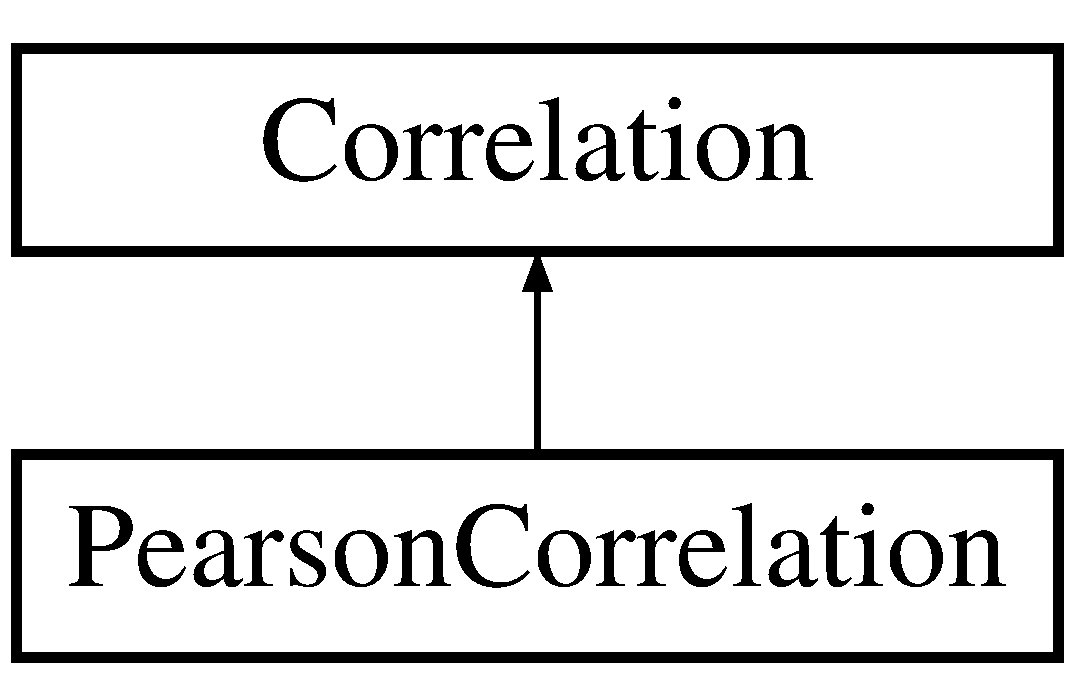
\includegraphics[height=2.000000cm]{classDataTools_1_1correlation_1_1PearsonCorrelation}
\end{center}
\end{figure}
\subsubsection*{Public Member Functions}
\begin{DoxyCompactItemize}
\item 
\mbox{\Hypertarget{classDataTools_1_1correlation_1_1PearsonCorrelation_afaeef6d70f6c46171dbd457e3c61c0b8}\label{classDataTools_1_1correlation_1_1PearsonCorrelation_afaeef6d70f6c46171dbd457e3c61c0b8}} 
{\bfseries Pearson\+Correlation} (I\+Enumerable$<$ \hyperlink{classDataTools_1_1Vector2}{Vector2} $>$ data)
\item 
\mbox{\Hypertarget{classDataTools_1_1correlation_1_1PearsonCorrelation_afff258bf05afa59c8fd4118e650e1682}\label{classDataTools_1_1correlation_1_1PearsonCorrelation_afff258bf05afa59c8fd4118e650e1682}} 
override double {\bfseries Get\+Correlation\+Coefficient} ()
\end{DoxyCompactItemize}
\subsubsection*{Additional Inherited Members}

\hypertarget{classDataTools_1_1regression_1_1PolynomialRegression}{}\subsection{Polynomial\+Regression Class Reference}
\label{classDataTools_1_1regression_1_1PolynomialRegression}\index{Polynomial\+Regression@{Polynomial\+Regression}}
\subsubsection*{Public Member Functions}
\begin{DoxyCompactItemize}
\item 
\mbox{\Hypertarget{classDataTools_1_1regression_1_1PolynomialRegression_aa3fbc58ba143383d0871ad14f8002cfb}\label{classDataTools_1_1regression_1_1PolynomialRegression_aa3fbc58ba143383d0871ad14f8002cfb}} 
{\bfseries Polynomial\+Regression} (I\+Enumerable$<$ \hyperlink{classDataTools_1_1Vector2}{Vector2} $>$ data, int polynomial\+Degree)
\item 
\mbox{\Hypertarget{classDataTools_1_1regression_1_1PolynomialRegression_ac5389e13f7d514bdb1f86084410a7403}\label{classDataTools_1_1regression_1_1PolynomialRegression_ac5389e13f7d514bdb1f86084410a7403}} 
double {\bfseries Predict\+Point} (double x)
\item 
\mbox{\Hypertarget{classDataTools_1_1regression_1_1PolynomialRegression_a5d4cd56b06140a849034cbc8622893ac}\label{classDataTools_1_1regression_1_1PolynomialRegression_a5d4cd56b06140a849034cbc8622893ac}} 
\hyperlink{classDataTools_1_1GenericVector}{Generic\+Vector} \mbox{[}$\,$\mbox{]} {\bfseries Get\+Polynomial\+Points} ()
\end{DoxyCompactItemize}

\hypertarget{classDataTools_1_1utils_1_1PriorityQue}{}\subsection{Priority\+Que$<$ T $>$ Class Template Reference}
\label{classDataTools_1_1utils_1_1PriorityQue}\index{Priority\+Que$<$ T $>$@{Priority\+Que$<$ T $>$}}
\subsubsection*{Public Member Functions}
\begin{DoxyCompactItemize}
\item 
\mbox{\Hypertarget{classDataTools_1_1utils_1_1PriorityQue_a71333bb99314f4112f3d79b75fba83cf}\label{classDataTools_1_1utils_1_1PriorityQue_a71333bb99314f4112f3d79b75fba83cf}} 
{\bfseries Priority\+Que} (I\+Enumerable$<$ Tuple$<$ double, T $>$$>$ entry)
\item 
\mbox{\Hypertarget{classDataTools_1_1utils_1_1PriorityQue_ab824f9a104dc1a7623f5803d8dfced87}\label{classDataTools_1_1utils_1_1PriorityQue_ab824f9a104dc1a7623f5803d8dfced87}} 
void {\bfseries Insert} (double priority, T que\+Item)
\item 
\mbox{\Hypertarget{classDataTools_1_1utils_1_1PriorityQue_aae3e6be1e179db7597e45466290dd6b0}\label{classDataTools_1_1utils_1_1PriorityQue_aae3e6be1e179db7597e45466290dd6b0}} 
\hyperlink{classDataTools_1_1utils_1_1QueItem}{Que\+Item}$<$ T $>$ {\bfseries Peek} ()
\item 
\mbox{\Hypertarget{classDataTools_1_1utils_1_1PriorityQue_a0a49e76c3c4756a635bbe7c55add2afa}\label{classDataTools_1_1utils_1_1PriorityQue_a0a49e76c3c4756a635bbe7c55add2afa}} 
\hyperlink{classDataTools_1_1utils_1_1QueItem}{Que\+Item}$<$ T $>$ {\bfseries Pop} ()
\item 
\mbox{\Hypertarget{classDataTools_1_1utils_1_1PriorityQue_ac075b80510e235ba9703b8a8c610275a}\label{classDataTools_1_1utils_1_1PriorityQue_ac075b80510e235ba9703b8a8c610275a}} 
List$<$ Tuple$<$ double, T $>$ $>$ {\bfseries To\+List} ()
\end{DoxyCompactItemize}
\subsubsection*{Public Attributes}
\begin{DoxyCompactItemize}
\item 
\mbox{\Hypertarget{classDataTools_1_1utils_1_1PriorityQue_aad462966ed963f892117056de1eba502}\label{classDataTools_1_1utils_1_1PriorityQue_aad462966ed963f892117056de1eba502}} 
int {\bfseries Count} =$>$ \+\_\+entries.\+Count
\item 
\mbox{\Hypertarget{classDataTools_1_1utils_1_1PriorityQue_aaaa6c7dd3bd14dc2ce7f0780de528bb1}\label{classDataTools_1_1utils_1_1PriorityQue_aaaa6c7dd3bd14dc2ce7f0780de528bb1}} 
bool {\bfseries Is\+Empty} =$>$ Count == 0
\end{DoxyCompactItemize}
\subsubsection*{Private Attributes}
\begin{DoxyCompactItemize}
\item 
\mbox{\Hypertarget{classDataTools_1_1utils_1_1PriorityQue_a8609f6bfdd54fdeff8e1f4ae6fadbe5e}\label{classDataTools_1_1utils_1_1PriorityQue_a8609f6bfdd54fdeff8e1f4ae6fadbe5e}} 
List$<$ Tuple$<$ double, T $>$ $>$ {\bfseries \+\_\+entries}
\end{DoxyCompactItemize}

\hypertarget{classDataTools_1_1utils_1_1QueItem}{}\subsection{Que\+Item$<$ T $>$ Class Template Reference}
\label{classDataTools_1_1utils_1_1QueItem}\index{Que\+Item$<$ T $>$@{Que\+Item$<$ T $>$}}
\subsubsection*{Public Member Functions}
\begin{DoxyCompactItemize}
\item 
\mbox{\Hypertarget{classDataTools_1_1utils_1_1QueItem_aec640d3f850f25436538b7b8d239dfa0}\label{classDataTools_1_1utils_1_1QueItem_aec640d3f850f25436538b7b8d239dfa0}} 
{\bfseries Que\+Item} (Tuple$<$ double, T $>$ que\+Item)
\end{DoxyCompactItemize}
\subsubsection*{Public Attributes}
\begin{DoxyCompactItemize}
\item 
\mbox{\Hypertarget{classDataTools_1_1utils_1_1QueItem_a1df2408757f0d8d500537d26c948fb0c}\label{classDataTools_1_1utils_1_1QueItem_a1df2408757f0d8d500537d26c948fb0c}} 
double {\bfseries Priority} =$>$ \+\_\+que\+Item.\+Item1
\item 
\mbox{\Hypertarget{classDataTools_1_1utils_1_1QueItem_ae76754367b2a77c2bcde5342ad346a26}\label{classDataTools_1_1utils_1_1QueItem_ae76754367b2a77c2bcde5342ad346a26}} 
T {\bfseries Item} =$>$ \+\_\+que\+Item.\+Item2
\end{DoxyCompactItemize}

\hypertarget{classHighcharts_1_1Replacer}{}\subsection{Replacer Class Reference}
\label{classHighcharts_1_1Replacer}\index{Replacer@{Replacer}}
\subsubsection*{Static Public Attributes}
\begin{DoxyCompactItemize}
\item 
\mbox{\Hypertarget{classHighcharts_1_1Replacer_a5dace676ed4488f45f5851faf4f1fb2f}\label{classHighcharts_1_1Replacer_a5dace676ed4488f45f5851faf4f1fb2f}} 
static readonly \hyperlink{classHighcharts_1_1Replacer}{Replacer} {\bfseries Div\+Id} = new \hyperlink{classHighcharts_1_1Replacer}{Replacer}(\char`\"{}divid\char`\"{})
\item 
\mbox{\Hypertarget{classHighcharts_1_1Replacer_a29f636c1789eae7c6ca026b3cb160ce2}\label{classHighcharts_1_1Replacer_a29f636c1789eae7c6ca026b3cb160ce2}} 
static readonly \hyperlink{classHighcharts_1_1Replacer}{Replacer} {\bfseries Chart} = new \hyperlink{classHighcharts_1_1Replacer}{Replacer}(\char`\"{}chart\char`\"{})
\item 
\mbox{\Hypertarget{classHighcharts_1_1Replacer_a3be5d0ad416935a20ec78b6d17531f5d}\label{classHighcharts_1_1Replacer_a3be5d0ad416935a20ec78b6d17531f5d}} 
static readonly \hyperlink{classHighcharts_1_1Replacer}{Replacer} {\bfseries Title} = new \hyperlink{classHighcharts_1_1Replacer}{Replacer}(\char`\"{}title\char`\"{})
\item 
\mbox{\Hypertarget{classHighcharts_1_1Replacer_a87e86b9f31233bc9cd9dbd3a43baf3f1}\label{classHighcharts_1_1Replacer_a87e86b9f31233bc9cd9dbd3a43baf3f1}} 
static readonly \hyperlink{classHighcharts_1_1Replacer}{Replacer} {\bfseries Subtitle} = new \hyperlink{classHighcharts_1_1Replacer}{Replacer}(\char`\"{}subtitle\char`\"{})
\item 
\mbox{\Hypertarget{classHighcharts_1_1Replacer_ac2709d3d7237a737809fad8d72ad57a8}\label{classHighcharts_1_1Replacer_ac2709d3d7237a737809fad8d72ad57a8}} 
static readonly \hyperlink{classHighcharts_1_1Replacer}{Replacer} {\bfseries Xlabel} = new \hyperlink{classHighcharts_1_1Replacer}{Replacer}(\char`\"{}xlabel\char`\"{})
\item 
\mbox{\Hypertarget{classHighcharts_1_1Replacer_a3f74a9d3e0f6b6bb93aac9d4ba30c8cc}\label{classHighcharts_1_1Replacer_a3f74a9d3e0f6b6bb93aac9d4ba30c8cc}} 
static readonly \hyperlink{classHighcharts_1_1Replacer}{Replacer} {\bfseries Ylabel} = new \hyperlink{classHighcharts_1_1Replacer}{Replacer}(\char`\"{}ylabel\char`\"{})
\item 
\mbox{\Hypertarget{classHighcharts_1_1Replacer_aeb6f8d0d38f280410865706032c317bd}\label{classHighcharts_1_1Replacer_aeb6f8d0d38f280410865706032c317bd}} 
static readonly \hyperlink{classHighcharts_1_1Replacer}{Replacer} {\bfseries Xtooltip} = new \hyperlink{classHighcharts_1_1Replacer}{Replacer}(\char`\"{}xtooltip\char`\"{})
\item 
\mbox{\Hypertarget{classHighcharts_1_1Replacer_aa5e813b3a470a67079475649f889835c}\label{classHighcharts_1_1Replacer_aa5e813b3a470a67079475649f889835c}} 
static readonly \hyperlink{classHighcharts_1_1Replacer}{Replacer} {\bfseries Ytooltip} = new \hyperlink{classHighcharts_1_1Replacer}{Replacer}(\char`\"{}ytooltip\char`\"{})
\item 
\mbox{\Hypertarget{classHighcharts_1_1Replacer_a52d1f0bff1a408bbf9c666a46099f821}\label{classHighcharts_1_1Replacer_a52d1f0bff1a408bbf9c666a46099f821}} 
static readonly \hyperlink{classHighcharts_1_1Replacer}{Replacer} {\bfseries Data} = new \hyperlink{classHighcharts_1_1Replacer}{Replacer}(\char`\"{}data\char`\"{})
\item 
\mbox{\Hypertarget{classHighcharts_1_1Replacer_a8122a2330b8cfeb8c78cdc5cf35e2de8}\label{classHighcharts_1_1Replacer_a8122a2330b8cfeb8c78cdc5cf35e2de8}} 
static readonly \hyperlink{classHighcharts_1_1Replacer}{Replacer} {\bfseries Type} = new \hyperlink{classHighcharts_1_1Replacer}{Replacer}(\char`\"{}type\char`\"{})
\item 
\mbox{\Hypertarget{classHighcharts_1_1Replacer_a8c5268c2c4eca614cb2f65e8d0e2b663}\label{classHighcharts_1_1Replacer_a8c5268c2c4eca614cb2f65e8d0e2b663}} 
static readonly \hyperlink{classHighcharts_1_1Replacer}{Replacer} {\bfseries Name} = new \hyperlink{classHighcharts_1_1Replacer}{Replacer}(\char`\"{}name\char`\"{})
\item 
\mbox{\Hypertarget{classHighcharts_1_1Replacer_a20e54647f393c33a98b462a8b58150ea}\label{classHighcharts_1_1Replacer_a20e54647f393c33a98b462a8b58150ea}} 
static readonly \hyperlink{classHighcharts_1_1Replacer}{Replacer} {\bfseries Marker} = new \hyperlink{classHighcharts_1_1Replacer}{Replacer}(\char`\"{}marker\char`\"{})
\item 
\mbox{\Hypertarget{classHighcharts_1_1Replacer_aa90e20f20aa31ed3377d49392063e356}\label{classHighcharts_1_1Replacer_aa90e20f20aa31ed3377d49392063e356}} 
static readonly \hyperlink{classHighcharts_1_1Replacer}{Replacer} {\bfseries Mousetracking} = new \hyperlink{classHighcharts_1_1Replacer}{Replacer}(\char`\"{}mousetracking\char`\"{})
\end{DoxyCompactItemize}
\subsubsection*{Properties}
\begin{DoxyCompactItemize}
\item 
\mbox{\Hypertarget{classHighcharts_1_1Replacer_af7b88db799d8f791f785e437bc6099d2}\label{classHighcharts_1_1Replacer_af7b88db799d8f791f785e437bc6099d2}} 
string {\bfseries Value}\hspace{0.3cm}{\ttfamily  \mbox{[}get\mbox{]}}
\end{DoxyCompactItemize}
\subsubsection*{Private Member Functions}
\begin{DoxyCompactItemize}
\item 
\mbox{\Hypertarget{classHighcharts_1_1Replacer_aad10b0644e2d606c7208a4600476be8b}\label{classHighcharts_1_1Replacer_aad10b0644e2d606c7208a4600476be8b}} 
{\bfseries Replacer} (string value)
\end{DoxyCompactItemize}

\hypertarget{classHighcharts_1_1Resources}{}\subsection{Resources Class Reference}
\label{classHighcharts_1_1Resources}\index{Resources@{Resources}}


Resource manager for the Assembly class.  


\subsubsection*{Static Public Member Functions}
\begin{DoxyCompactItemize}
\item 
\mbox{\Hypertarget{classHighcharts_1_1Resources_ad3f81074aa73ae9bc68128f6bebc8ec9}\label{classHighcharts_1_1Resources_ad3f81074aa73ae9bc68128f6bebc8ec9}} 
static Stream {\bfseries Load\+File} (string resource)
\item 
\mbox{\Hypertarget{classHighcharts_1_1Resources_ada9fe61069360cd3ec9187f10bb5b947}\label{classHighcharts_1_1Resources_ada9fe61069360cd3ec9187f10bb5b947}} 
static string \mbox{[}$\,$\mbox{]} {\bfseries Get\+Resources\+Names} ()
\end{DoxyCompactItemize}
\subsubsection*{Static Private Attributes}
\begin{DoxyCompactItemize}
\item 
\mbox{\Hypertarget{classHighcharts_1_1Resources_a0eb1013cca2e8e9c882143930723fc75}\label{classHighcharts_1_1Resources_a0eb1013cca2e8e9c882143930723fc75}} 
static readonly Assembly {\bfseries Assembly} = typeof(\hyperlink{classHighcharts_1_1Highchart}{Highchart}).Get\+Type\+Info().Assembly
\end{DoxyCompactItemize}


\subsubsection{Detailed Description}
Resource manager for the Assembly class. 

This class manages the files that are copied in the assembly upon compilation. 
\hypertarget{classDataTools_1_1correlation_1_1SpearmanCorrelation}{}\subsection{Spearman\+Correlation Class Reference}
\label{classDataTools_1_1correlation_1_1SpearmanCorrelation}\index{Spearman\+Correlation@{Spearman\+Correlation}}
Inheritance diagram for Spearman\+Correlation\+:\begin{figure}[H]
\begin{center}
\leavevmode
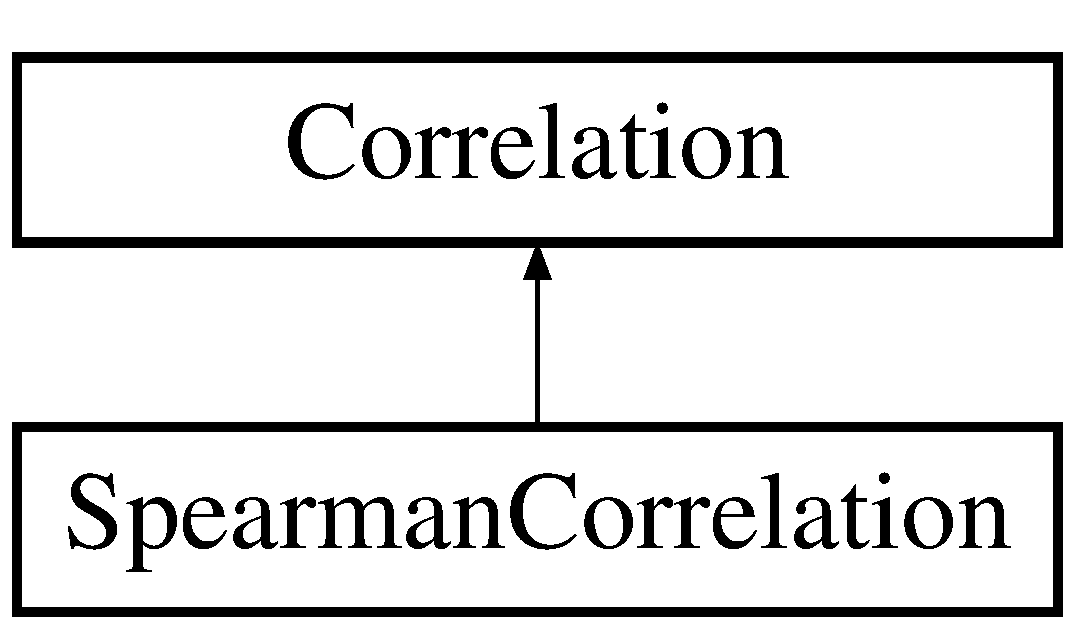
\includegraphics[height=2.000000cm]{classDataTools_1_1correlation_1_1SpearmanCorrelation}
\end{center}
\end{figure}
\subsubsection*{Public Member Functions}
\begin{DoxyCompactItemize}
\item 
\mbox{\Hypertarget{classDataTools_1_1correlation_1_1SpearmanCorrelation_a57c5b09341d60a6a06276a9a913474ba}\label{classDataTools_1_1correlation_1_1SpearmanCorrelation_a57c5b09341d60a6a06276a9a913474ba}} 
{\bfseries Spearman\+Correlation} (I\+Enumerable$<$ \hyperlink{classDataTools_1_1Vector2}{Vector2} $>$ data)
\item 
\mbox{\Hypertarget{classDataTools_1_1correlation_1_1SpearmanCorrelation_afff258bf05afa59c8fd4118e650e1682}\label{classDataTools_1_1correlation_1_1SpearmanCorrelation_afff258bf05afa59c8fd4118e650e1682}} 
override double {\bfseries Get\+Correlation\+Coefficient} ()
\end{DoxyCompactItemize}
\subsubsection*{Additional Inherited Members}

\hypertarget{classHighcharts_1_1TmplEngine}{}\subsection{Tmpl\+Engine Class Reference}
\label{classHighcharts_1_1TmplEngine}\index{Tmpl\+Engine@{Tmpl\+Engine}}
\subsubsection*{Static Public Member Functions}
\begin{DoxyCompactItemize}
\item 
\mbox{\Hypertarget{classHighcharts_1_1TmplEngine_a77654540d7c9217f0d90f4624b0c77f3}\label{classHighcharts_1_1TmplEngine_a77654540d7c9217f0d90f4624b0c77f3}} 
static string {\bfseries Create\+Template} (\hyperlink{interfaceHighcharts_1_1ITmplModel}{I\+Tmpl\+Model} model)
\end{DoxyCompactItemize}
\subsubsection*{Private Attributes}
\begin{DoxyCompactItemize}
\item 
\mbox{\Hypertarget{classHighcharts_1_1TmplEngine_a6121a594f50cd69a1b661a52b7346120}\label{classHighcharts_1_1TmplEngine_a6121a594f50cd69a1b661a52b7346120}} 
const string {\bfseries Prefix} = \char`\"{}Highcharts.\+Files.\char`\"{}
\item 
\mbox{\Hypertarget{classHighcharts_1_1TmplEngine_a5e958797e07b0bd922b59e561f05bb1f}\label{classHighcharts_1_1TmplEngine_a5e958797e07b0bd922b59e561f05bb1f}} 
const string {\bfseries File\+Extension} = \char`\"{}.tmpl\char`\"{}
\item 
\mbox{\Hypertarget{classHighcharts_1_1TmplEngine_ae81c1612fbd57f120c2c8e649755a23a}\label{classHighcharts_1_1TmplEngine_ae81c1612fbd57f120c2c8e649755a23a}} 
const string {\bfseries Left\+Token} = \char`\"{}$<$\%\char`\"{}
\item 
\mbox{\Hypertarget{classHighcharts_1_1TmplEngine_acd06761bcd01254df6e1915c9ab2b79a}\label{classHighcharts_1_1TmplEngine_acd06761bcd01254df6e1915c9ab2b79a}} 
const string {\bfseries Right\+Token} = \char`\"{}\%$>$\char`\"{}
\end{DoxyCompactItemize}

\hypertarget{classDataTools_1_1utils_1_1Utils}{}\subsection{Utils Class Reference}
\label{classDataTools_1_1utils_1_1Utils}\index{Utils@{Utils}}
\subsubsection*{Static Public Member Functions}
\begin{DoxyCompactItemize}
\item 
\mbox{\Hypertarget{classDataTools_1_1utils_1_1Utils_a9af52b94d12e047becd0cd5d335c8fbd}\label{classDataTools_1_1utils_1_1Utils_a9af52b94d12e047becd0cd5d335c8fbd}} 
static void {\bfseries Times} (this int count, System.\+Action action)
\end{DoxyCompactItemize}

\hypertarget{classDataTools_1_1Vector2}{}\subsection{Vector2 Class Reference}
\label{classDataTools_1_1Vector2}\index{Vector2@{Vector2}}


Two dimensional vector.  


\subsubsection*{Public Member Functions}
\begin{DoxyCompactItemize}
\item 
\mbox{\Hypertarget{classDataTools_1_1Vector2_a54f14911c467791709425b5816b5ef33}\label{classDataTools_1_1Vector2_a54f14911c467791709425b5816b5ef33}} 
{\bfseries Vector2} (double x, double y)
\end{DoxyCompactItemize}
\subsubsection*{Properties}
\begin{DoxyCompactItemize}
\item 
\mbox{\Hypertarget{classDataTools_1_1Vector2_a1059b82f84827fc49ea81b12566b3cdb}\label{classDataTools_1_1Vector2_a1059b82f84827fc49ea81b12566b3cdb}} 
double {\bfseries X}\hspace{0.3cm}{\ttfamily  \mbox{[}get, set\mbox{]}}
\item 
\mbox{\Hypertarget{classDataTools_1_1Vector2_ac8d59bf77d5ef21e7c7a88b08f14c825}\label{classDataTools_1_1Vector2_ac8d59bf77d5ef21e7c7a88b08f14c825}} 
double {\bfseries Y}\hspace{0.3cm}{\ttfamily  \mbox{[}get, set\mbox{]}}
\end{DoxyCompactItemize}


\subsubsection{Detailed Description}
Two dimensional vector. 

Two dimensional vector having a X and Y dimension. 
%--- End generated contents ---

% Index
\newpage
\phantomsection
\clearemptydoublepage
\addcontentsline{toc}{section}{Index}
\printindex

\end{document}
